\documentclass{article} % This command is used to set the type of document you are working on such as an article, book, or presenation

\usepackage{geometry} % This package allows the editing of the page layout
\usepackage{amsmath}  % This package allows the use of a large range of mathematical formula, commands, and symbols
\usepackage{graphicx}  % This package allows the importing of images

\newcommand{\question}[2][]{\begin{flushleft}\textbf{Question #1}: \textit{#2}\end{flushleft}}
\newcommand{\sol}{\textbf{Solution}:} %Use if you want a boldface solution line
\newcommand{\maketitletwo}[2][]{\begin{center}
        \Large{\textbf{Lab 1 Report}
        
            Deep Learning} % Name of course here
        \vspace{5pt}
        
        \normalsize{
            Name: Kai-Jie Lin 
            
            Student ID: 110652019
            
            \today}
        \vspace{15pt}
        \end{center}}
\begin{document}
    \maketitletwo[5]  % Optional argument is assignment number
    %Keep a blank space between maketitletwo and \question[1]
    
    \section{Introduction}

    In this lab, I implemented a simple neural network using the Numpy library.
    The neural network was trained on the linear data and XOR data.
    I implemented the forward and backward propagation, linear layer, various activation functions(Sigmoid, ReLU) and optimizers(SGD, Adagrad, Momentum).
    The result of the neural network performs differently under different configurations.
    
    \section{Experiment setups}
    
    \subsection{Sigmoid functions}
    
    $$
    \sigma(x) = \frac{1}{1+e^{-x}} \quad
    \sigma'(x) = \sigma(x)(1-\sigma(x))
    $$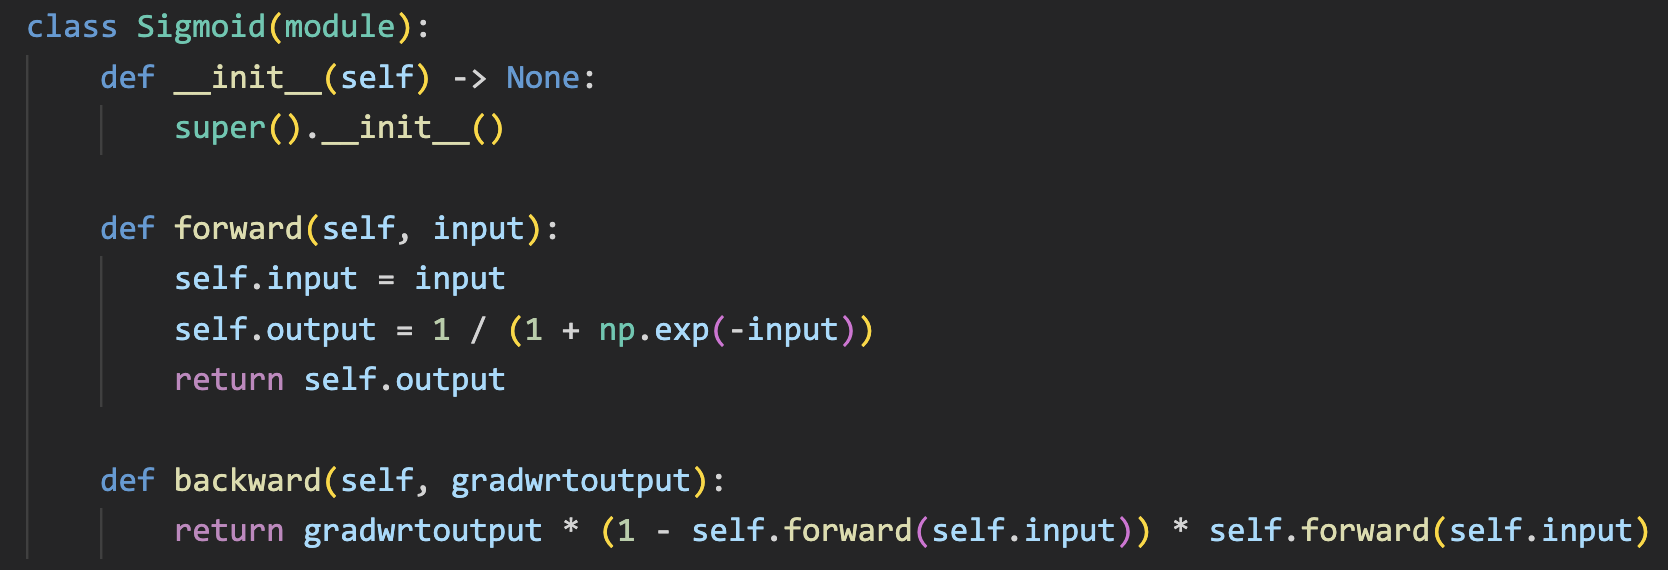
\includegraphics[width=13cm]{./imgs/sigmoid.png}

    \subsection{Neural network}

    $W_1, W_2, W_3$ are the random initialized weights of the neural network. $\sigma$ is the sigmoid function.
    
    \[
    \begin{aligned}
        a_1 &= W_1x \\
        b_1 &= \sigma(a_1) \\
        a_2 &= W_2b_1 \\
        b_2 &= \sigma(a_2) \\
        a_3 &= W_3b_2 \\
        \hat{y} &= \sigma(a_3) \\
    \end{aligned}
    \]Self defined linear layer module: \\
    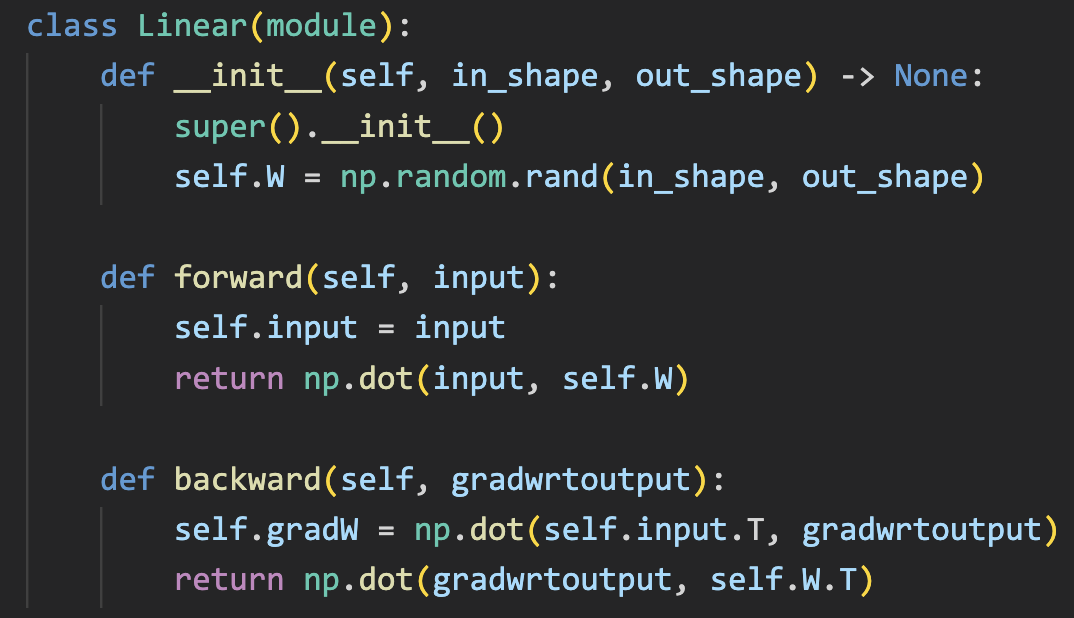
\includegraphics[width=10cm]{./imgs/linear.png} \\
    Forward part of the neural network: \\
    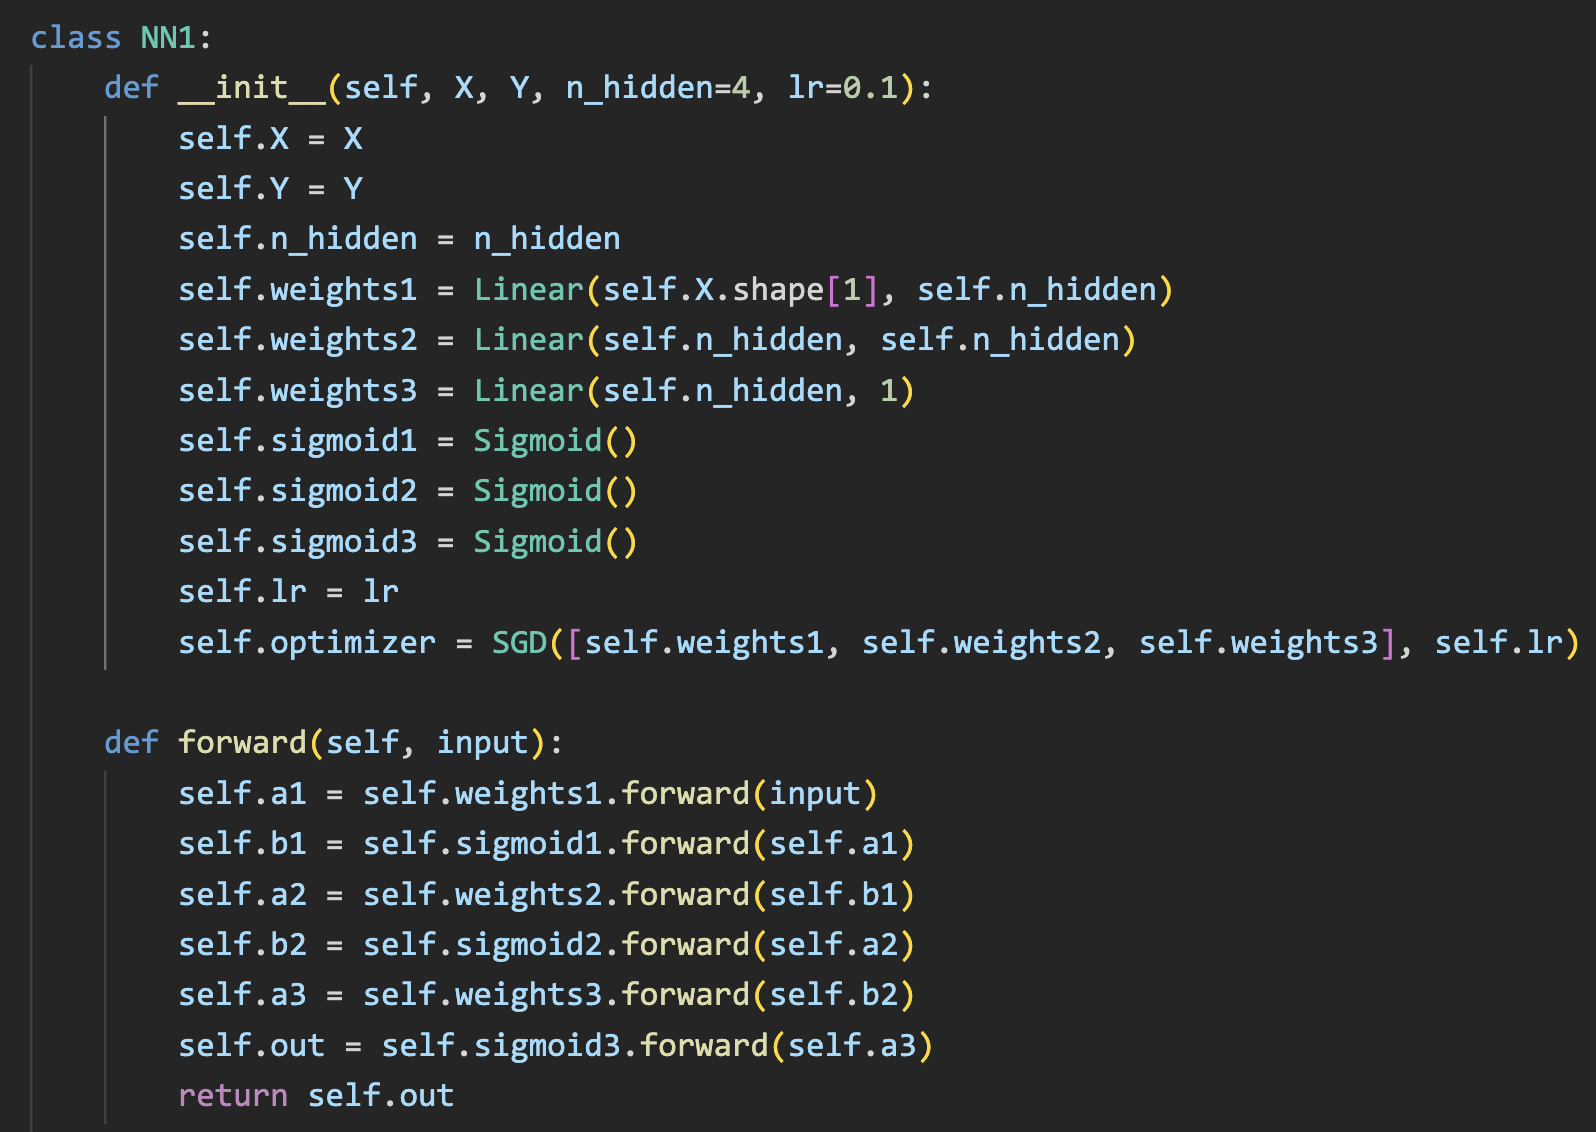
\includegraphics[width=14cm]{./imgs/nn.png} \\
    

    \subsection{Backpropagation}
    $L$ is loss of forward propagation. $\hat{y}$ is the output of the neural network.
    \[
    \begin{aligned}
    \frac{\partial L}{\partial W_3} &= \frac{\partial \hat{y}}{\partial W_3} \frac{\partial L}{\partial \hat{y}} \\
    \frac{\partial L}{\partial W_2} &= \frac{\partial b_2}{\partial W_2} \frac{\partial \hat{y}}{\partial b_2} \frac{\partial L}{\partial \hat{y}} \\
    \frac{\partial L}{\partial W_1} &= \frac{\partial b_1}{\partial W_1} \frac{\partial b_2}{\partial b_1} \frac{\partial \hat{y}}{\partial b_2} \frac{\partial L}{\partial \hat{y}} \\
    \end{aligned}
    \]Use Stochastic Gradient Descent(SGD) to update the weights. \\
    \[
    W_1 = W_1 - \alpha \frac{\partial L}{\partial W_1} \quad
    W_2 = W_2 - \alpha \frac{\partial L}{\partial W_2} \quad
    W_3 = W_3 - \alpha \frac{\partial L}{\partial W_3} \quad
    \]Every linear layer and activation functions have a backward function to calculate the gradients. \\
    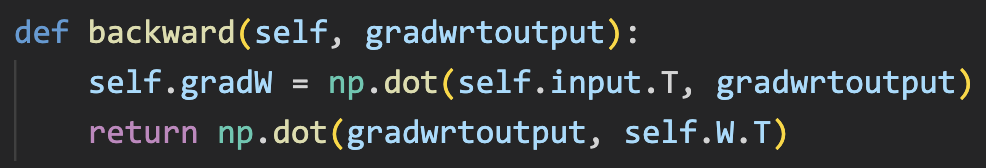
\includegraphics[width=10cm]{./imgs/linear_back.png} \\
    We can easily get the gradients of the weights by chain rule. \\
    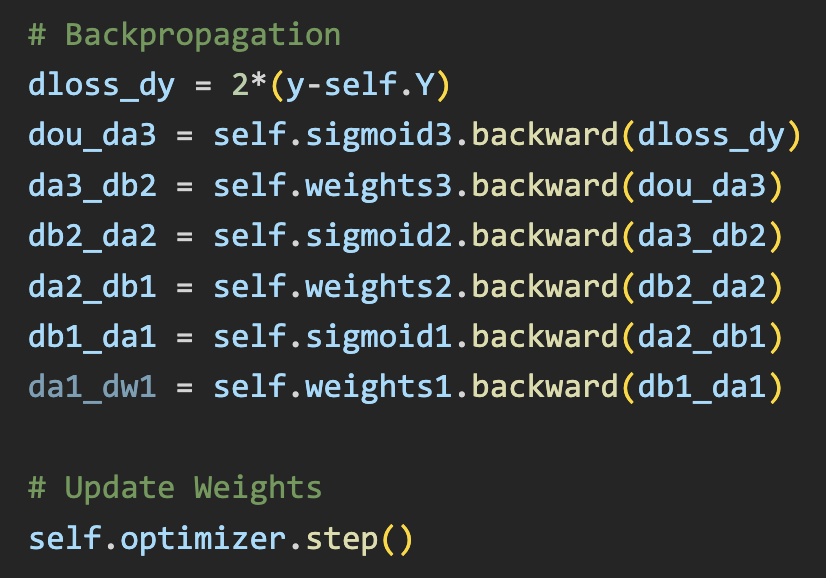
\includegraphics[width=9cm]{./imgs/backprop.png} \\
    Finally, we can update the weights by SGD. \\
    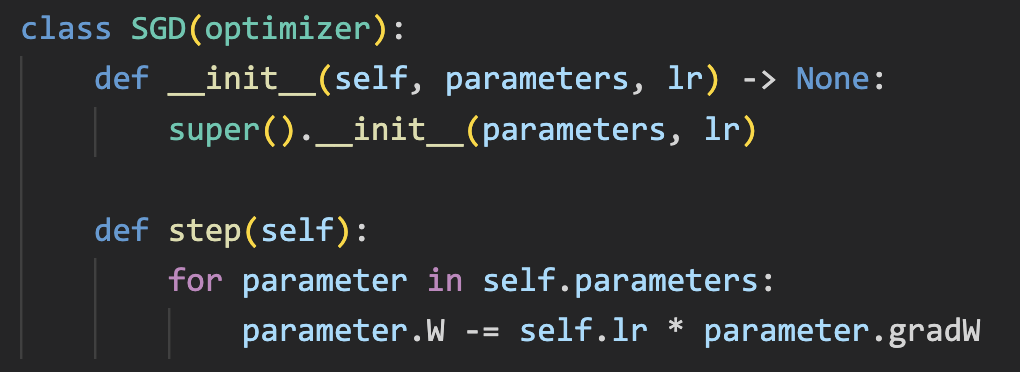
\includegraphics[width=9cm]{./imgs/SGD.png} \\

    \section{Results of testings}
    \textbf{Configurations:} \\
    2 Linear Layers \\ 
    4 Hidden Units \\
    Learning Rate: 0.1 \\
    Activation Function: Sigmoid \\
    Optimizer: SGD \\
    \subsection{Screenshot and comparison figure}
    Training Process(Linear Data): \\
    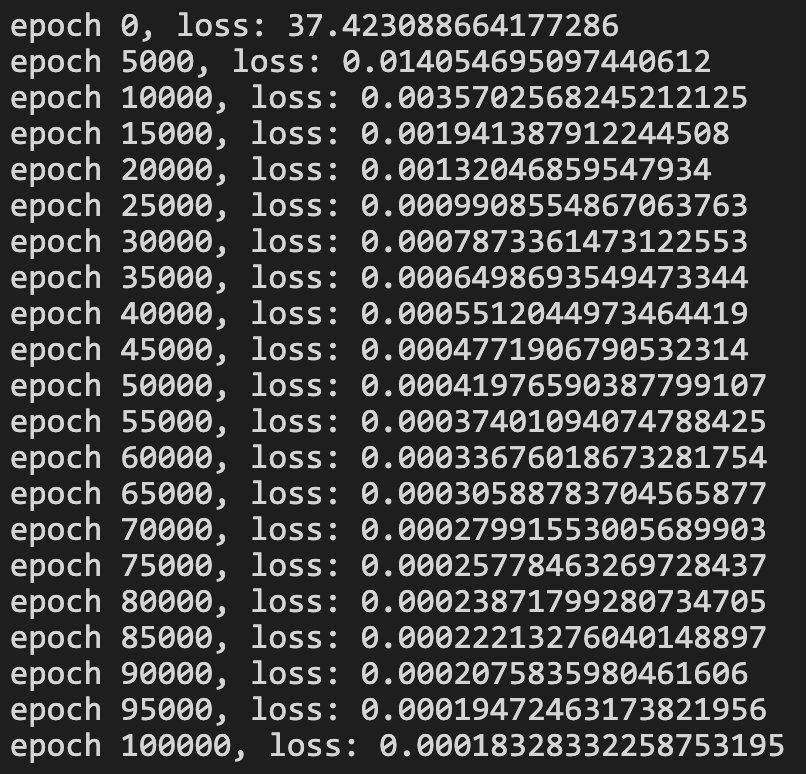
\includegraphics[width=6cm]{./imgs/linear_train.png} \\
    
    Training Process(XOR Data): \\
    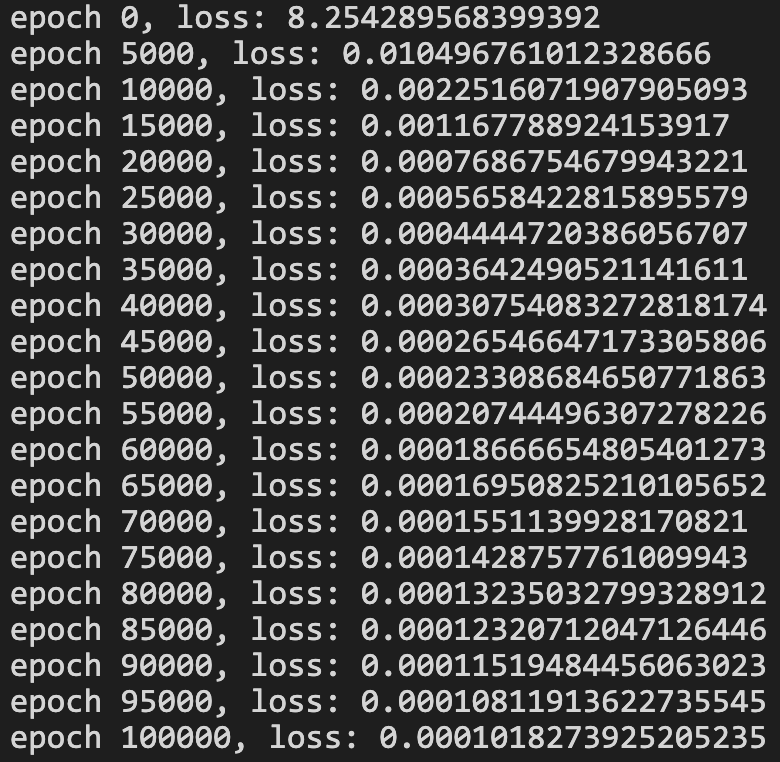
\includegraphics[width=6cm]{./imgs/xor_train.png} \\
     
    
    \subsection{Show the accuracy of your prediction}
    \textbf{Testing(Linear Data):} \\
    Accuracy: 100\% \\
    Result and prediction: \\
    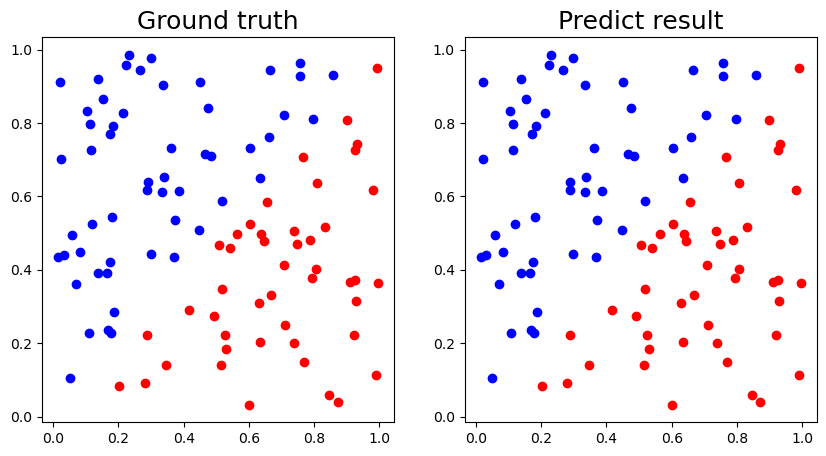
\includegraphics[width=10cm]{./imgs/linear_data.png} \\
    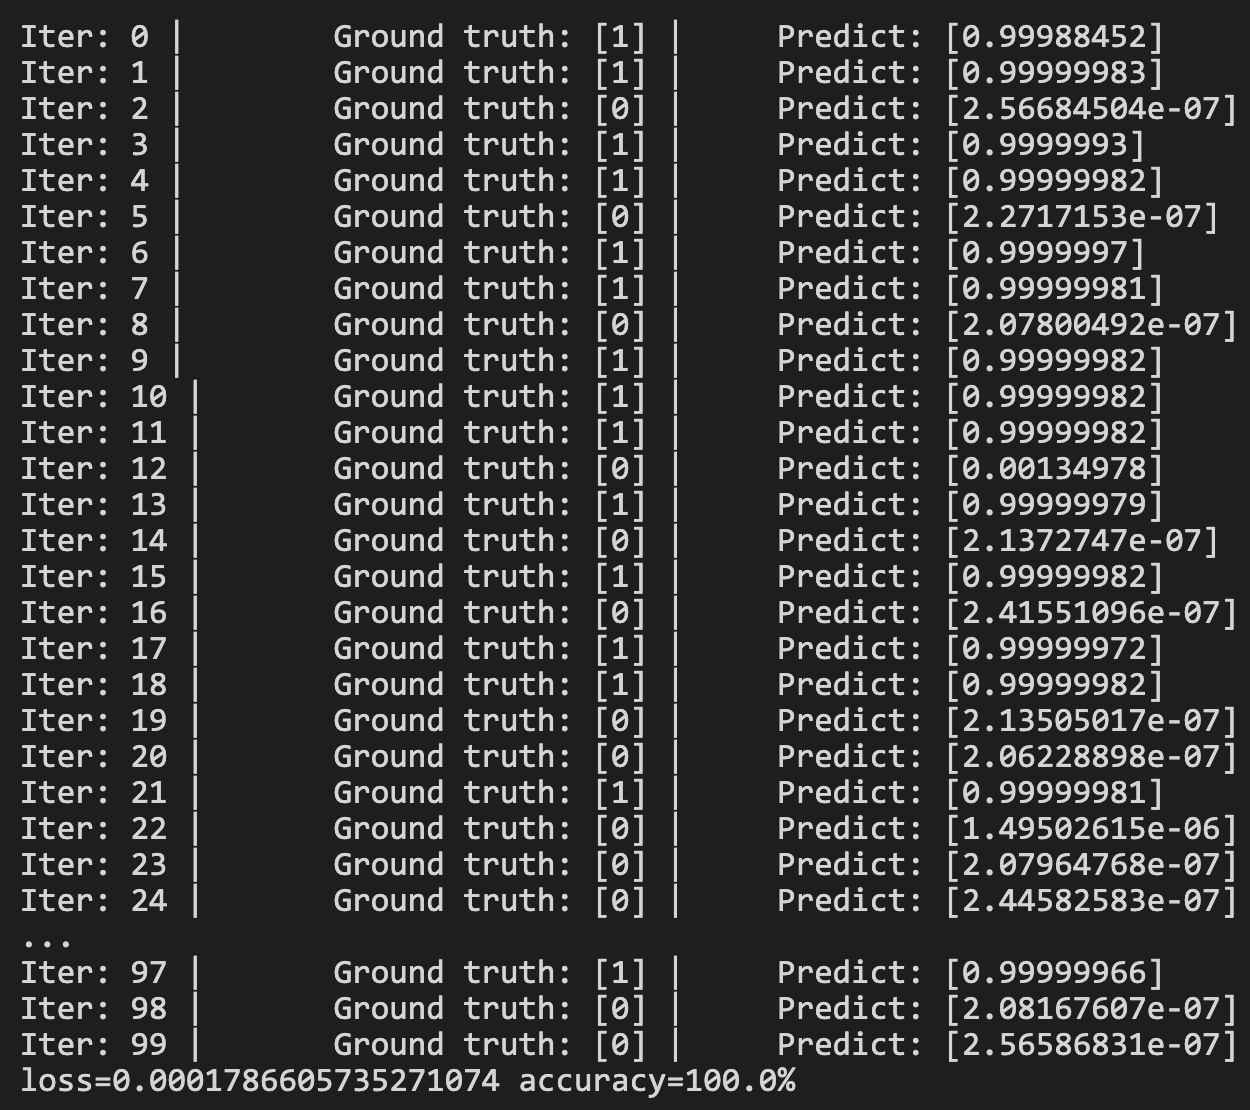
\includegraphics[width=7.5cm]{./imgs/linear_pred1.png} \\
    \textbf{Testing(XOR Data):} \\
    Accuracy: 100\% \\
    Result and prediction: \\
    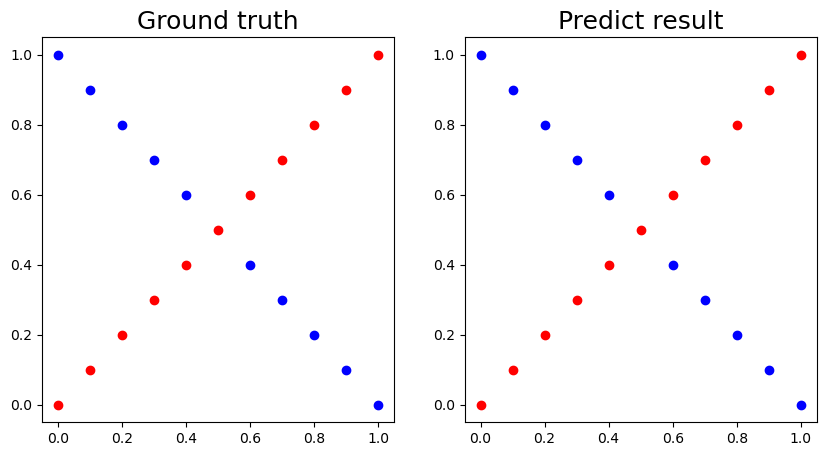
\includegraphics[width=10cm]{./imgs/xor.png} \\ 
    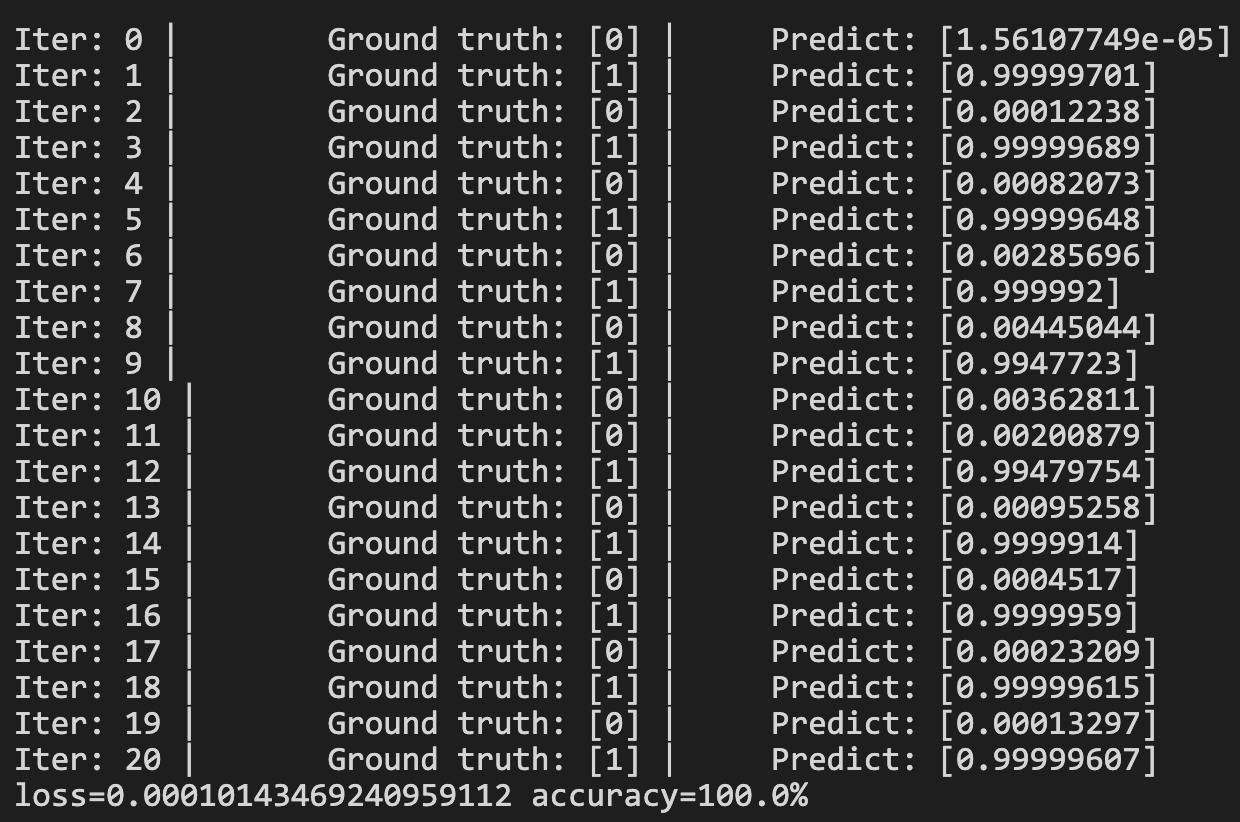
\includegraphics[width=7.5cm]{./imgs/xor_pred1.png} \\

    \subsection{Learning curve (loss, epoch curve)}
    \textbf{Learning curve (Left: Linear Data / Right: XOR data)} \\
    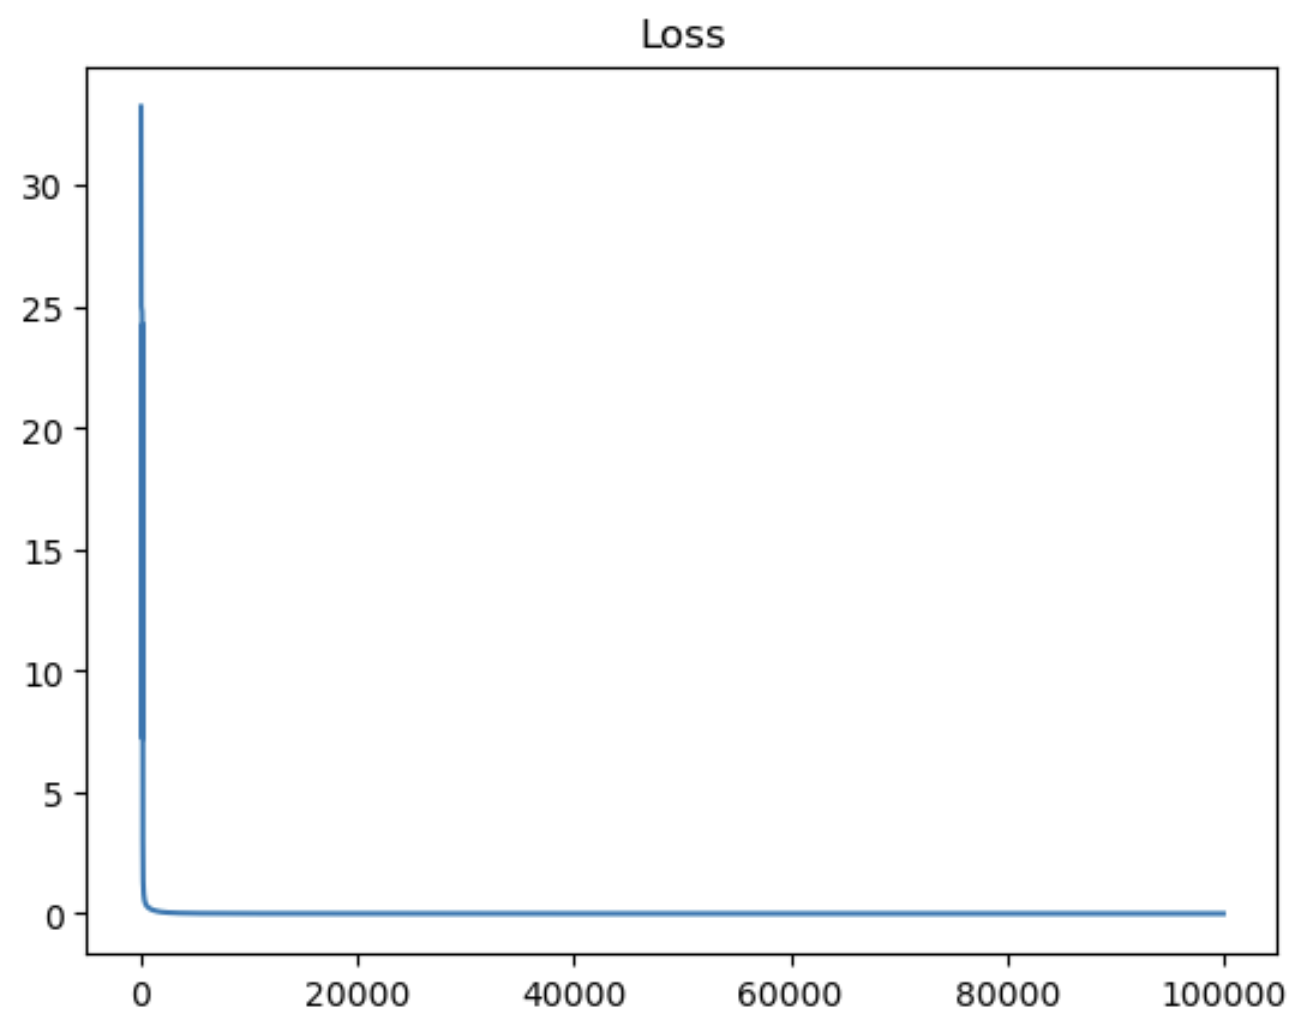
\includegraphics[width=7.5cm]{./imgs/linear_loss.png} 
    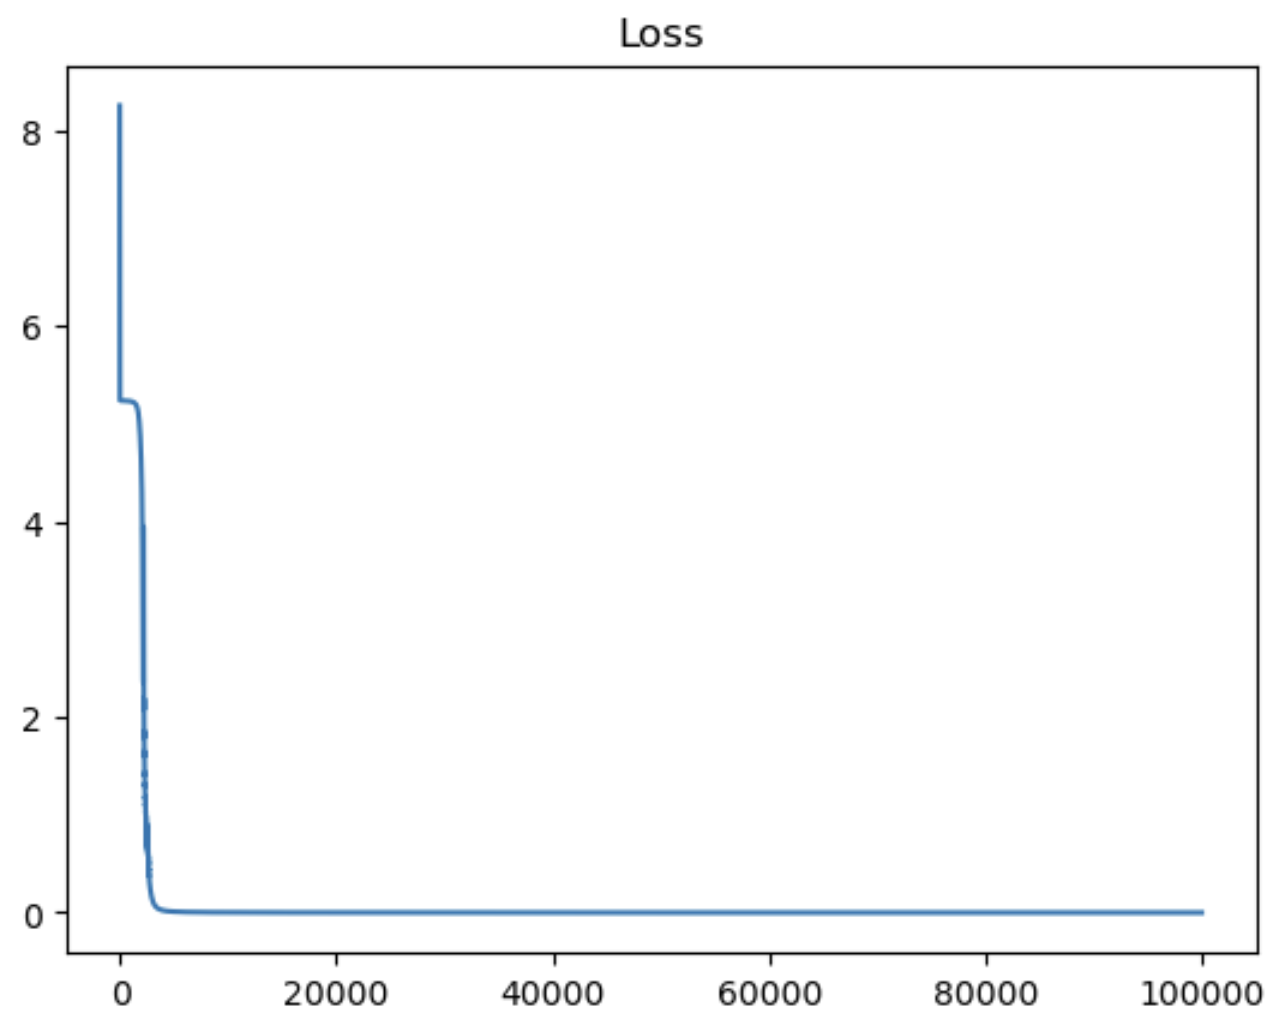
\includegraphics[width=7.5cm]{./imgs/xor_loss.png} \\
    
    \section{Discussion}
    
    \subsection{Different learning rates}
    \textbf{Linear Data:} \\
    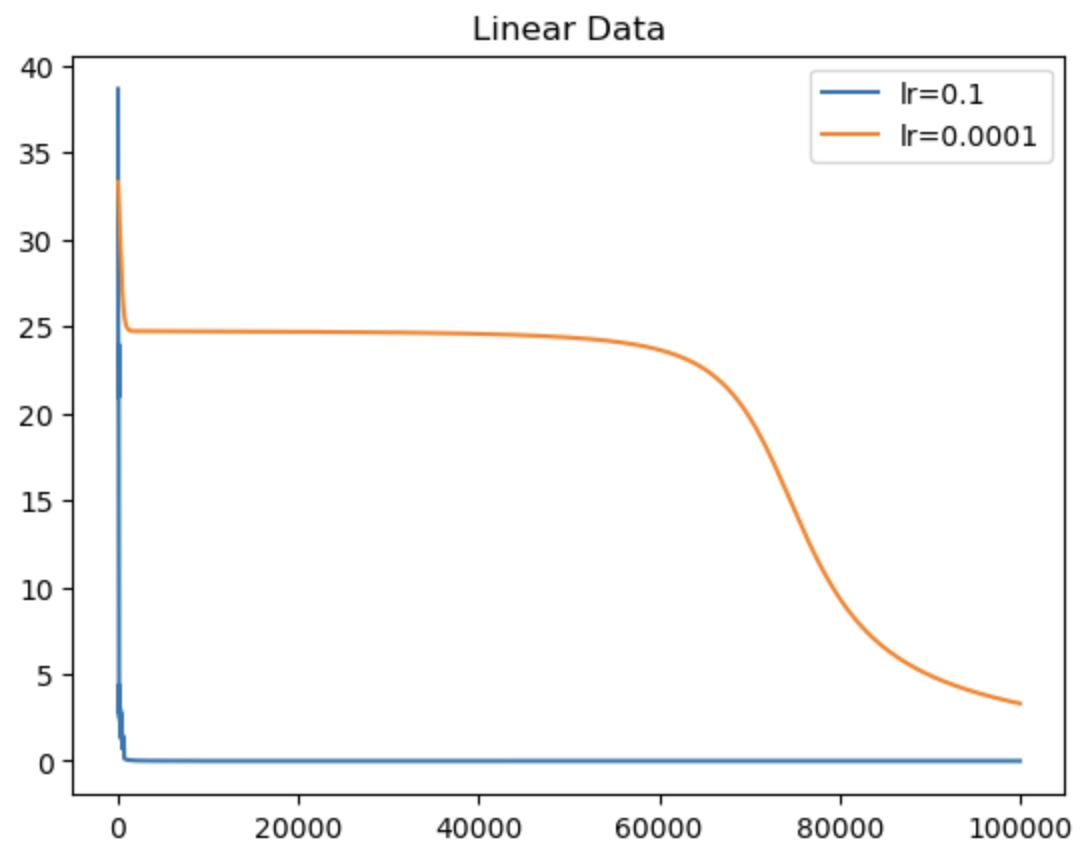
\includegraphics[width=7.5cm]{./imgs/linear_loss_cmp.png} \\
    We can find that the learning rate is too small, the loss will decrease slowly. The accuracy of lr=0.1 is 100\% and the accuracy
    of lr=0.0001 is 99\%. \\
    Prediction result(lr=0.1): \\
    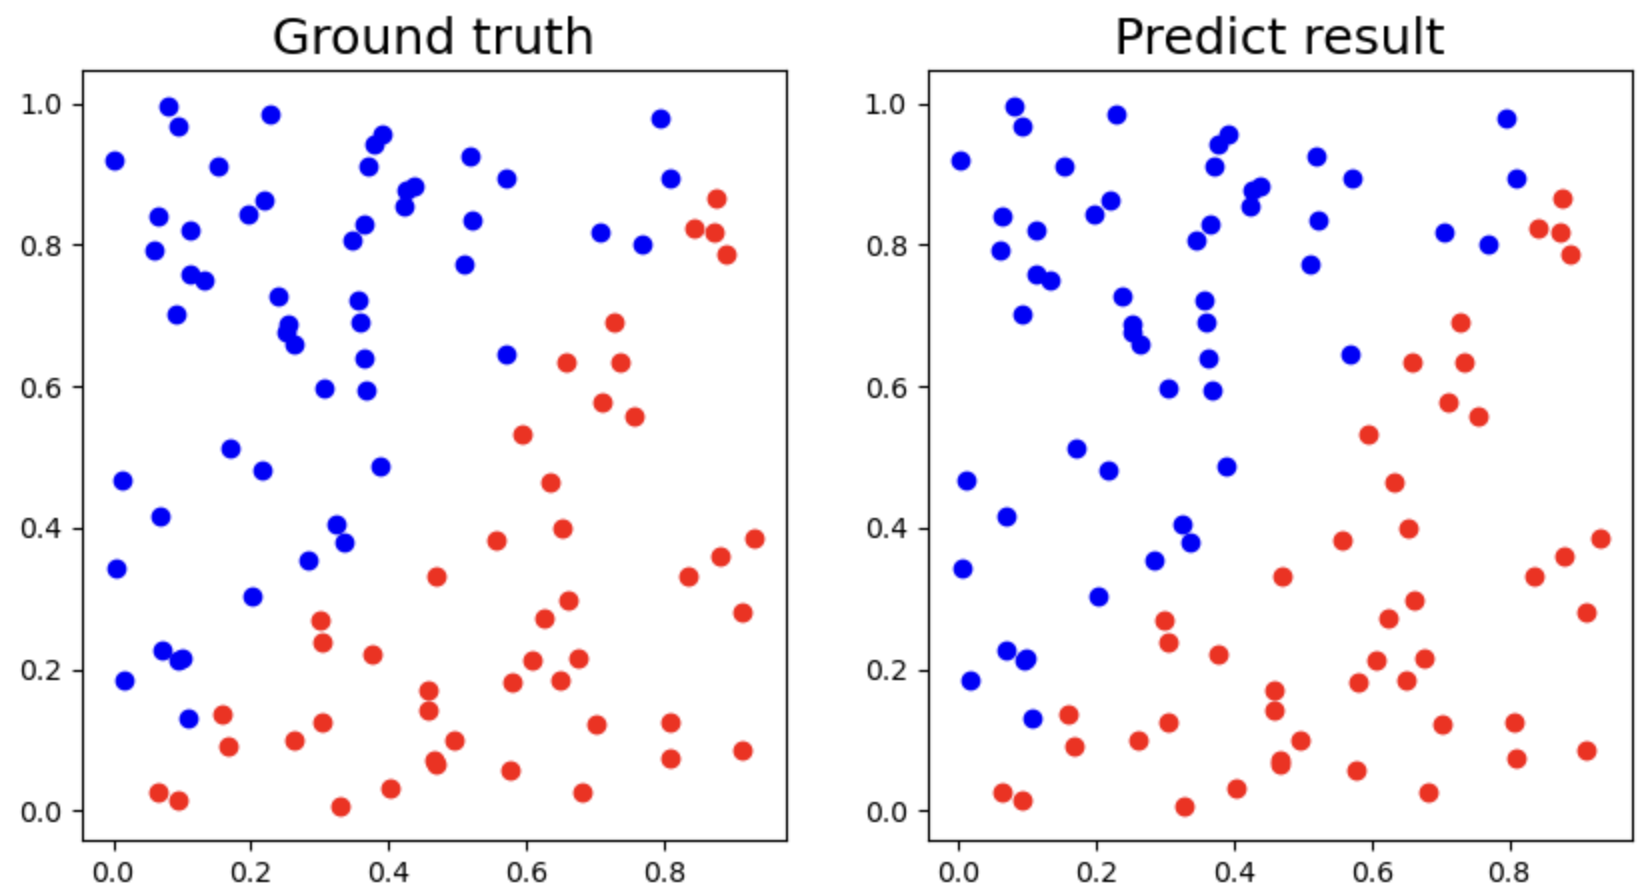
\includegraphics[width=7cm]{./imgs/linear_lr0.1.png} \\
    Prediction result(lr=0.0001): \\
    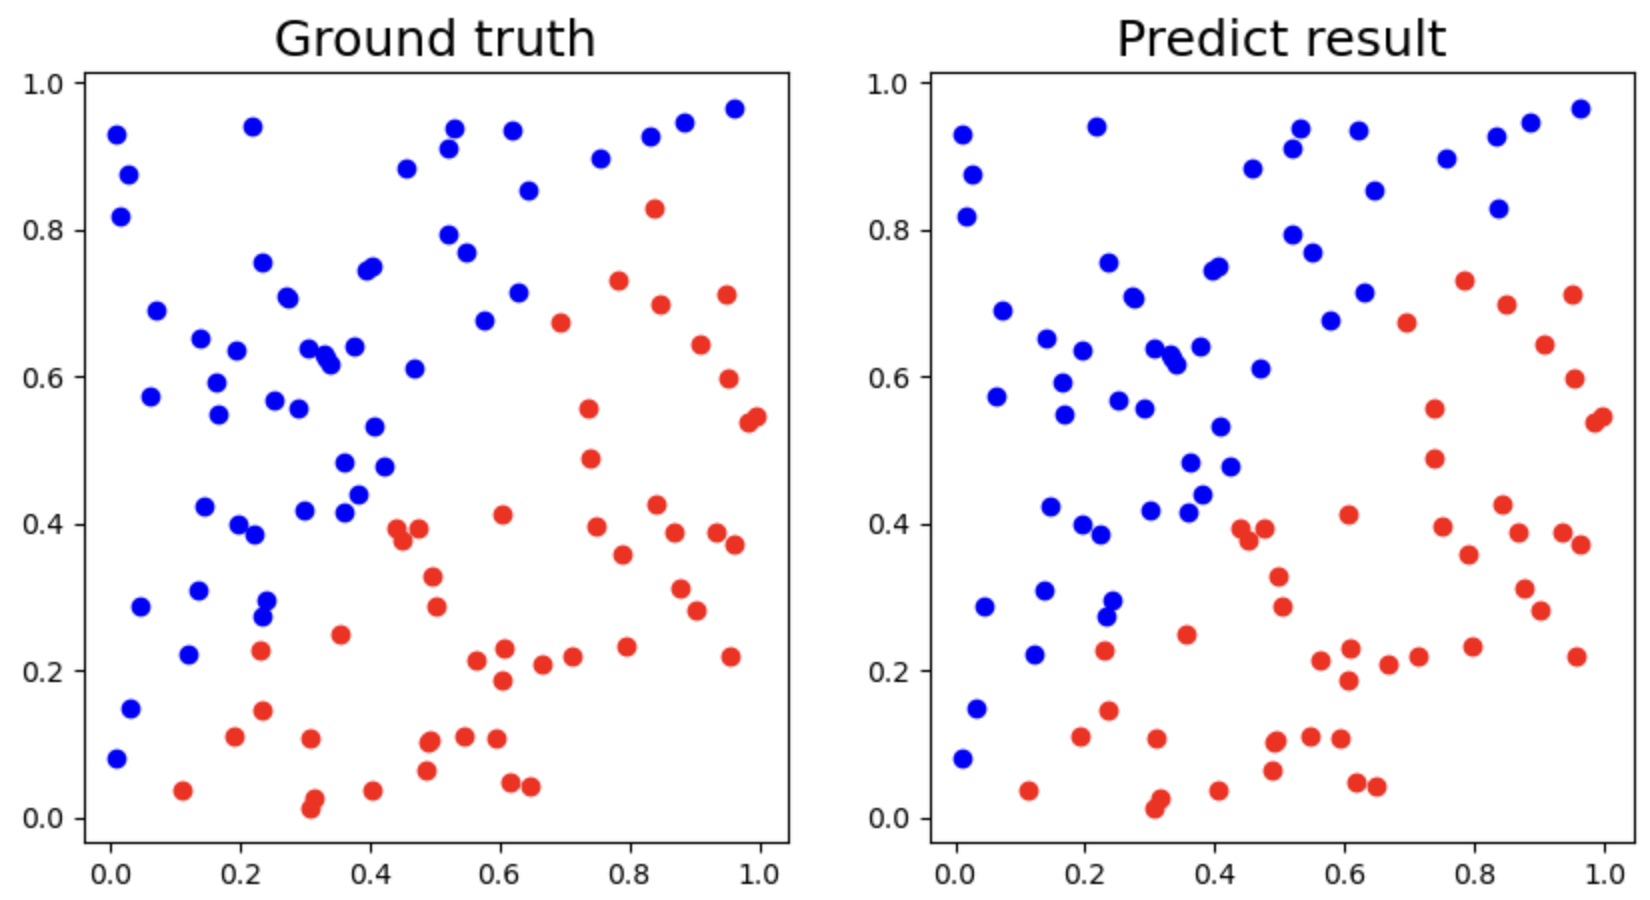
\includegraphics[width=7cm]{./imgs/linear_lr0.0001.png} \\

    \textbf{XOR Data:} \\
    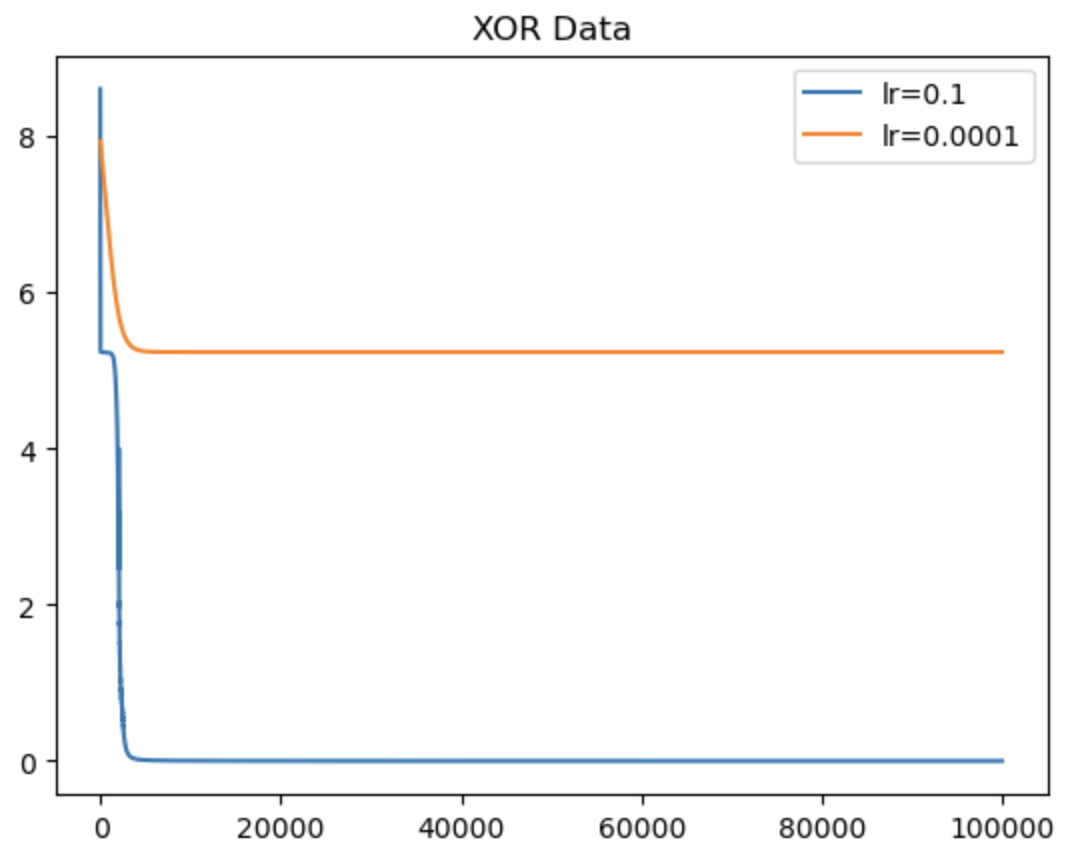
\includegraphics[width=7.5cm]{./imgs/xor_loss_cmp.png} \\
    We can find that the learning rate is too small, the loss will decrease slowly. The accuracy of lr=0.1 is 100\% and the accuracy
    of lr=0.0001 is 52\%. \\
    Prediction result(lr=0.1): \\
    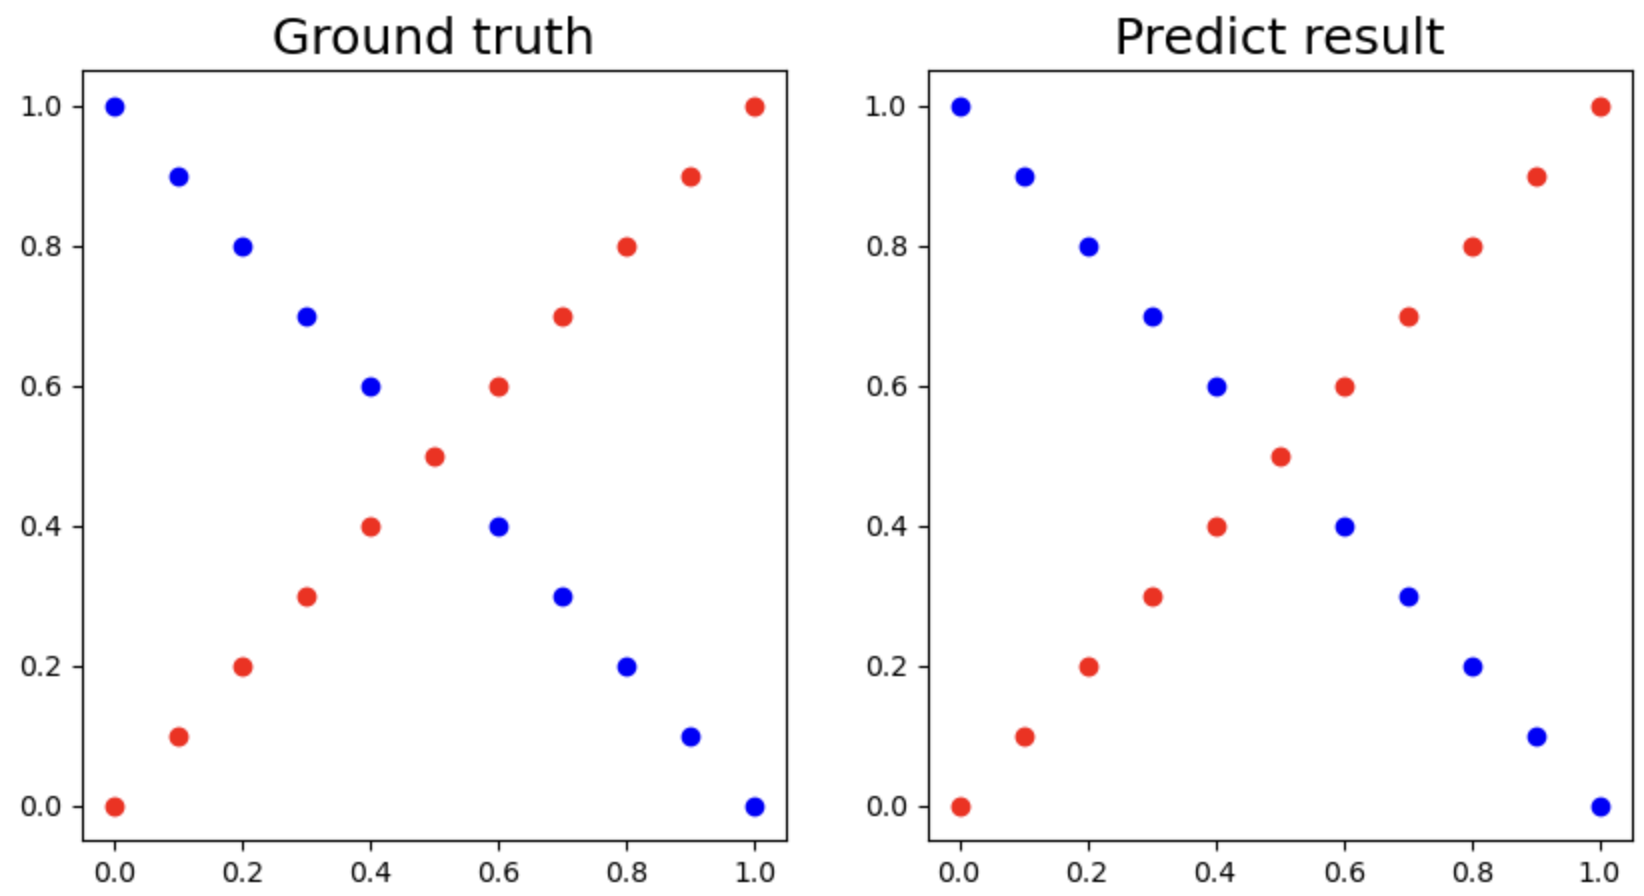
\includegraphics[width=7cm]{./imgs/xor_lr0.1.png} \\
    Prediction result(lr=0.0001): \\
    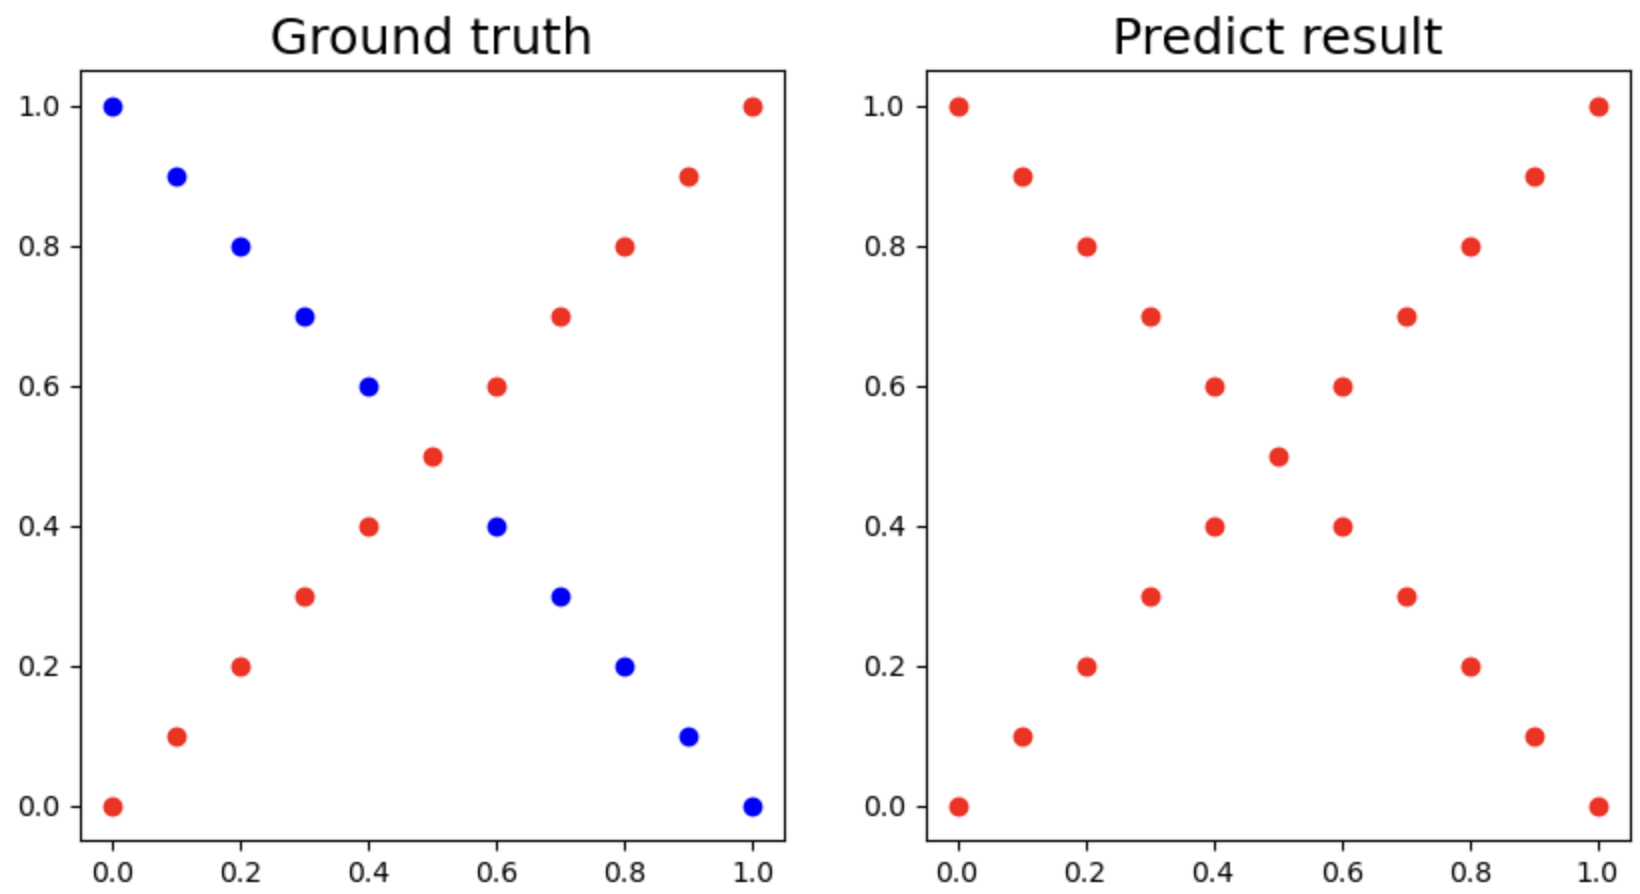
\includegraphics[width=7cm]{./imgs/xor_lr0.0001.png} \\
    
    \subsection{Different numbers of hidden units}
    We compare the loss and accuracy between 2 hidden units and 8 hidden units. \\
    \textbf{Linear Data:} \\
    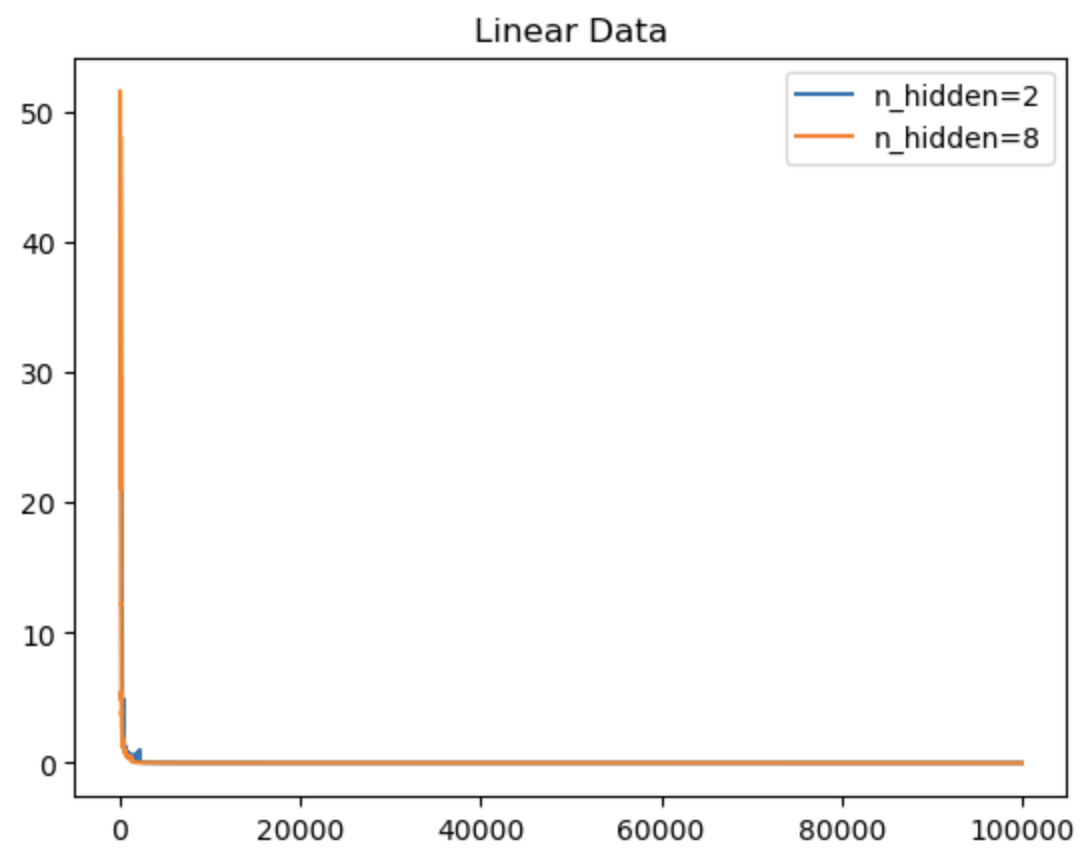
\includegraphics[width=7.5cm]{./imgs/linear_n_hidden.png} \\
    Both accuracies are 100\%. Numbers of hidden units do not affect the accuracy a lot. \\
    \textbf{XOR Data:} \\
    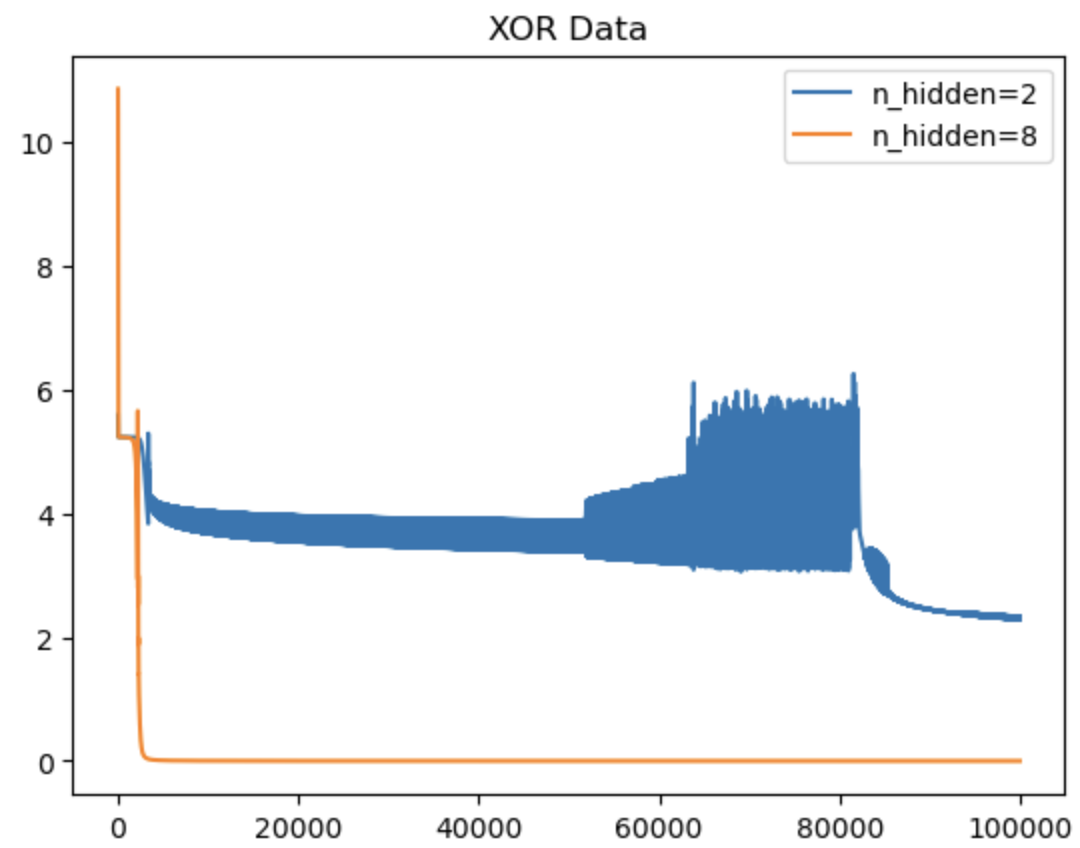
\includegraphics[width=7.5cm]{./imgs/xor_n_hidden.png} \\
    When number of hidden units is 2, the loss can not converge very well and the accuracy is only 72\%.
    But when the number of hidden units increase to 8, the loss can converge well and the accuracy is 100\%. \\
    
    \subsection{Try without activation functions}
    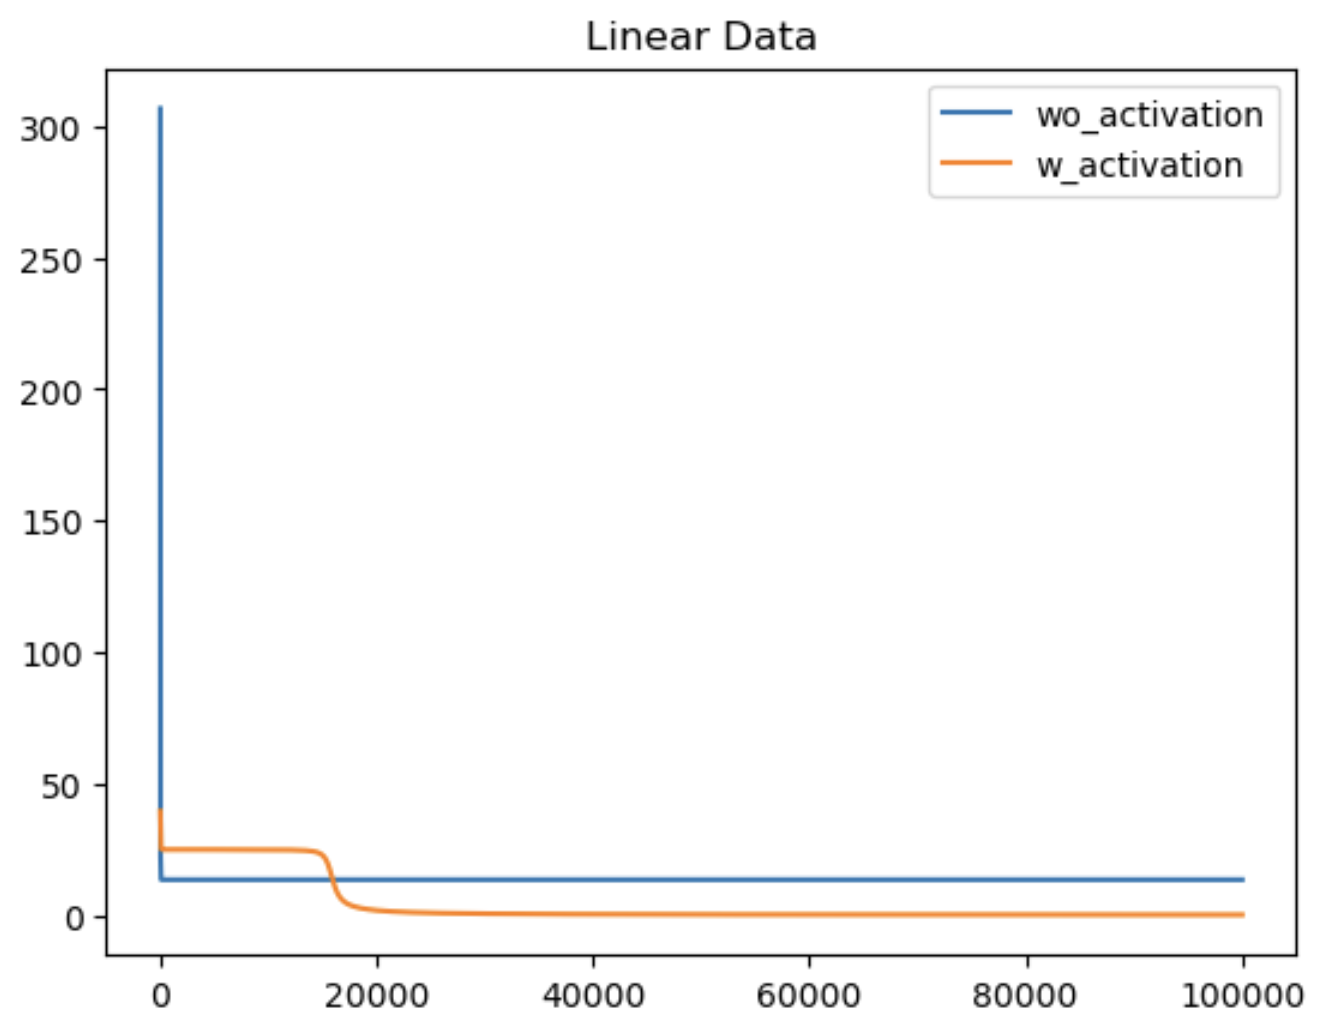
\includegraphics[width=7.5cm]{./imgs/wo_act_loss.png}
    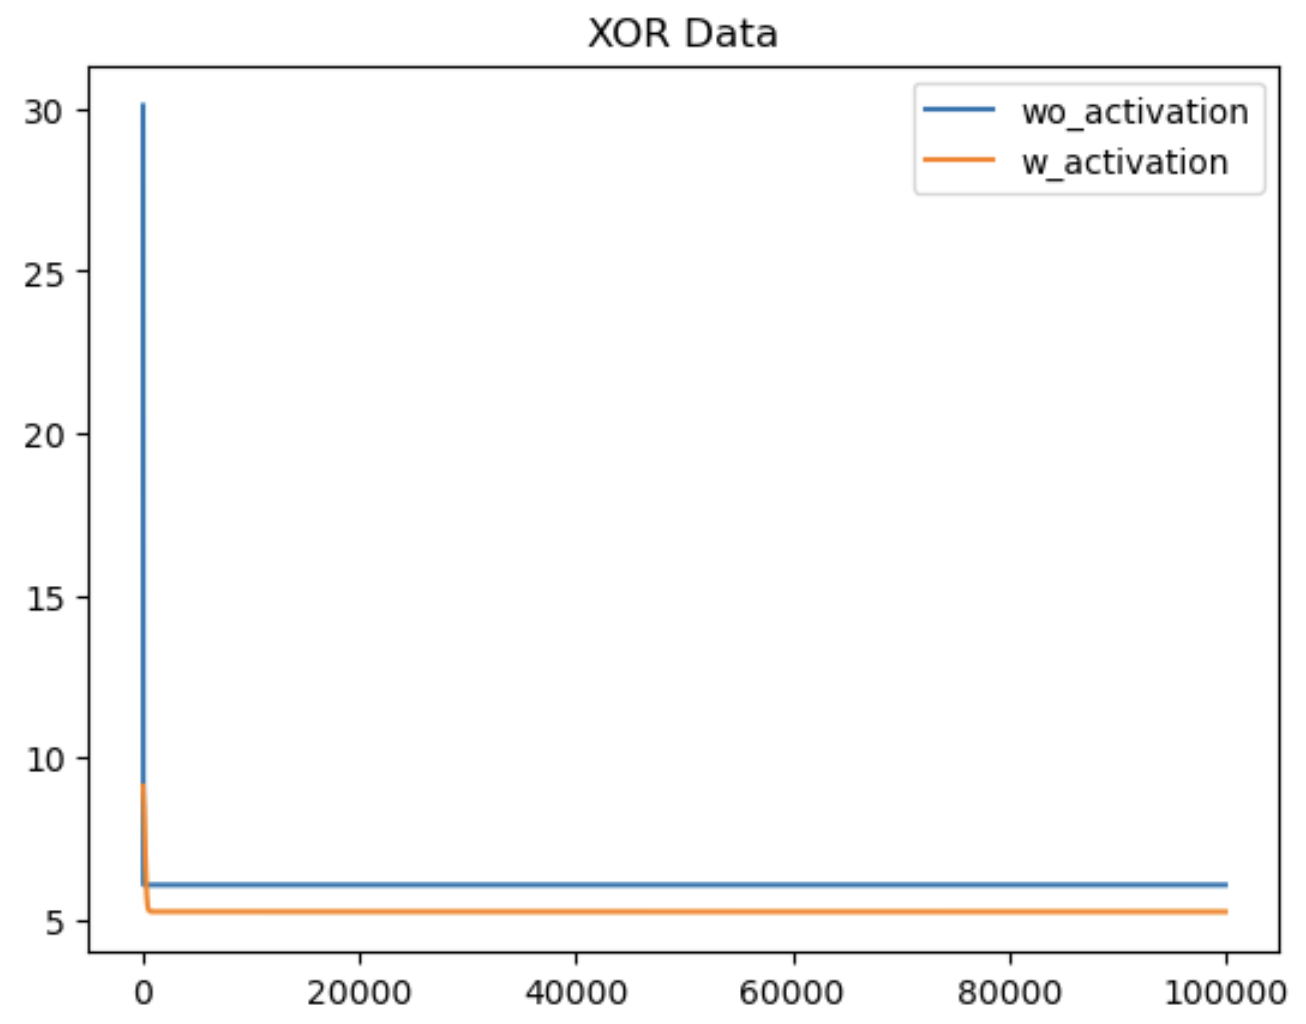
\includegraphics[width=7.5cm]{./imgs/xor_wo_act.png} \\
    The model can not learn very well without activation functions. I tuned the learning rate to 0.01 since if the learning rate is too large, the loss will explode without activation function.
    The accuracy of model without activation functions is only 88\% under linear data and 33\% under XOR data.

    \section{Extra}
    \subsection{Different activation functions}
    Implement ReLU activation function. \\
    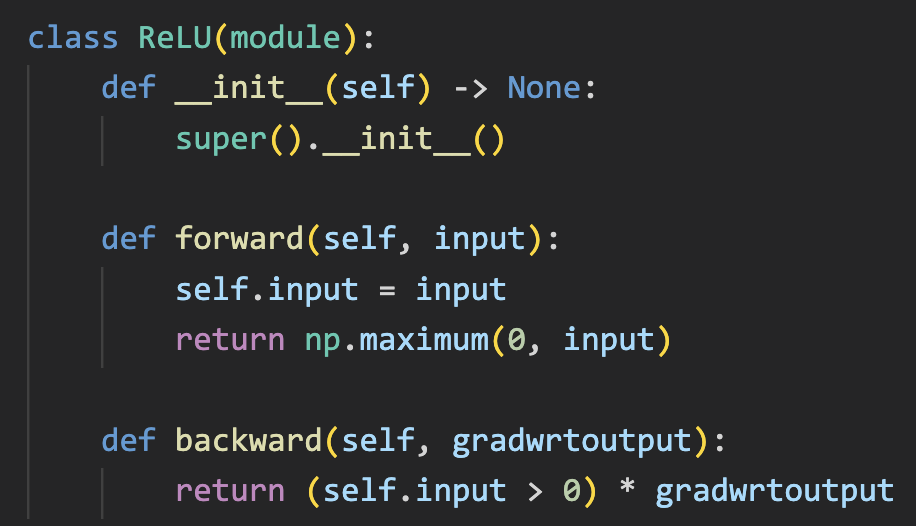
\includegraphics[width=7.5cm]{./imgs/relu.png} \\
    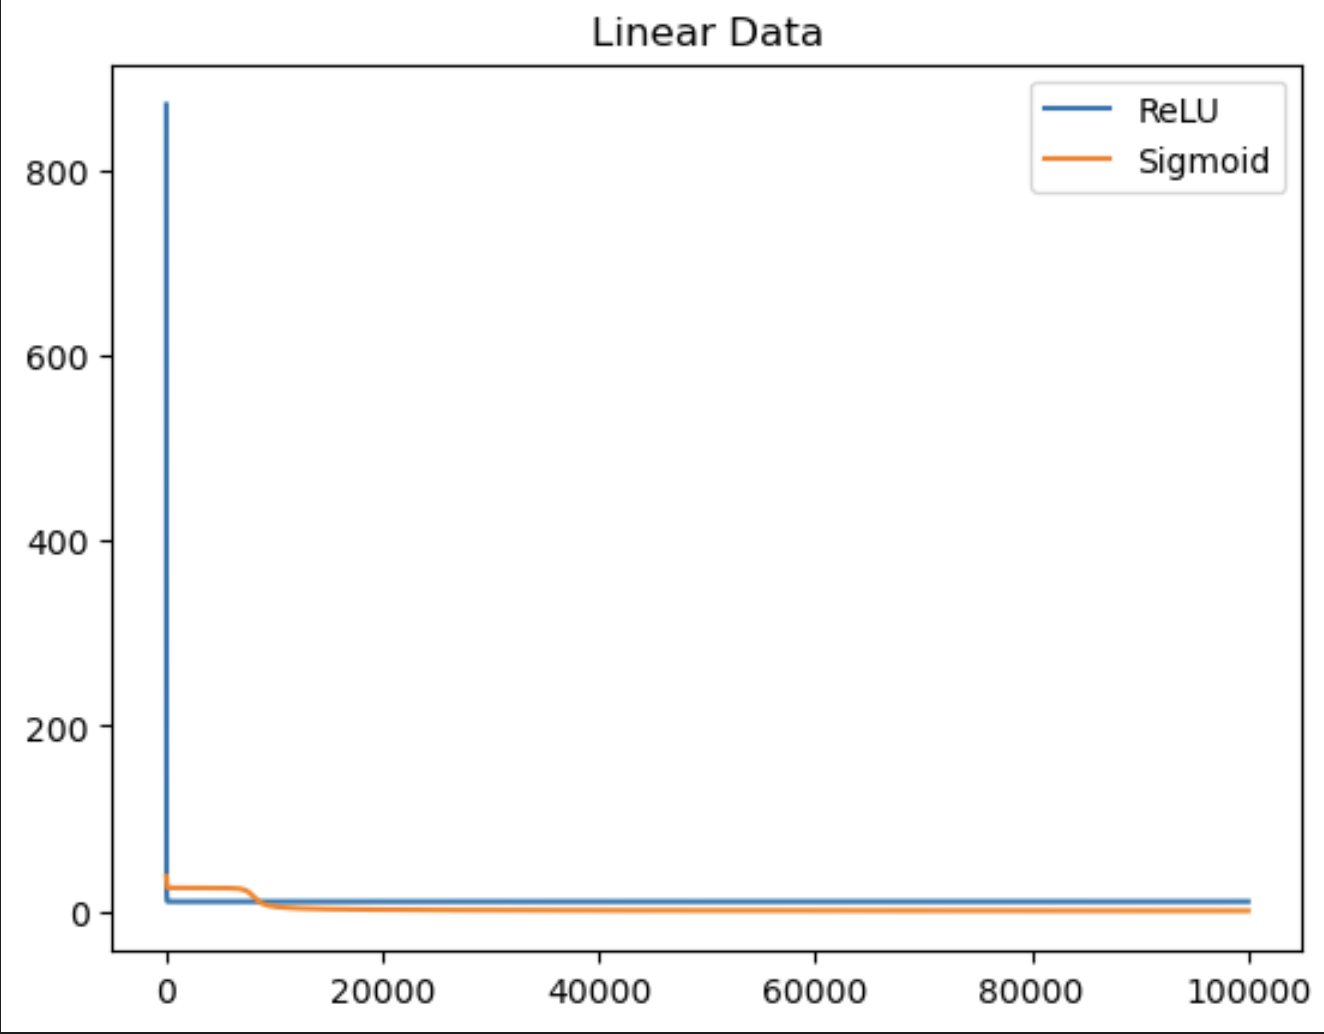
\includegraphics[width=7.5cm]{./imgs/linear_relu_loss.png}
    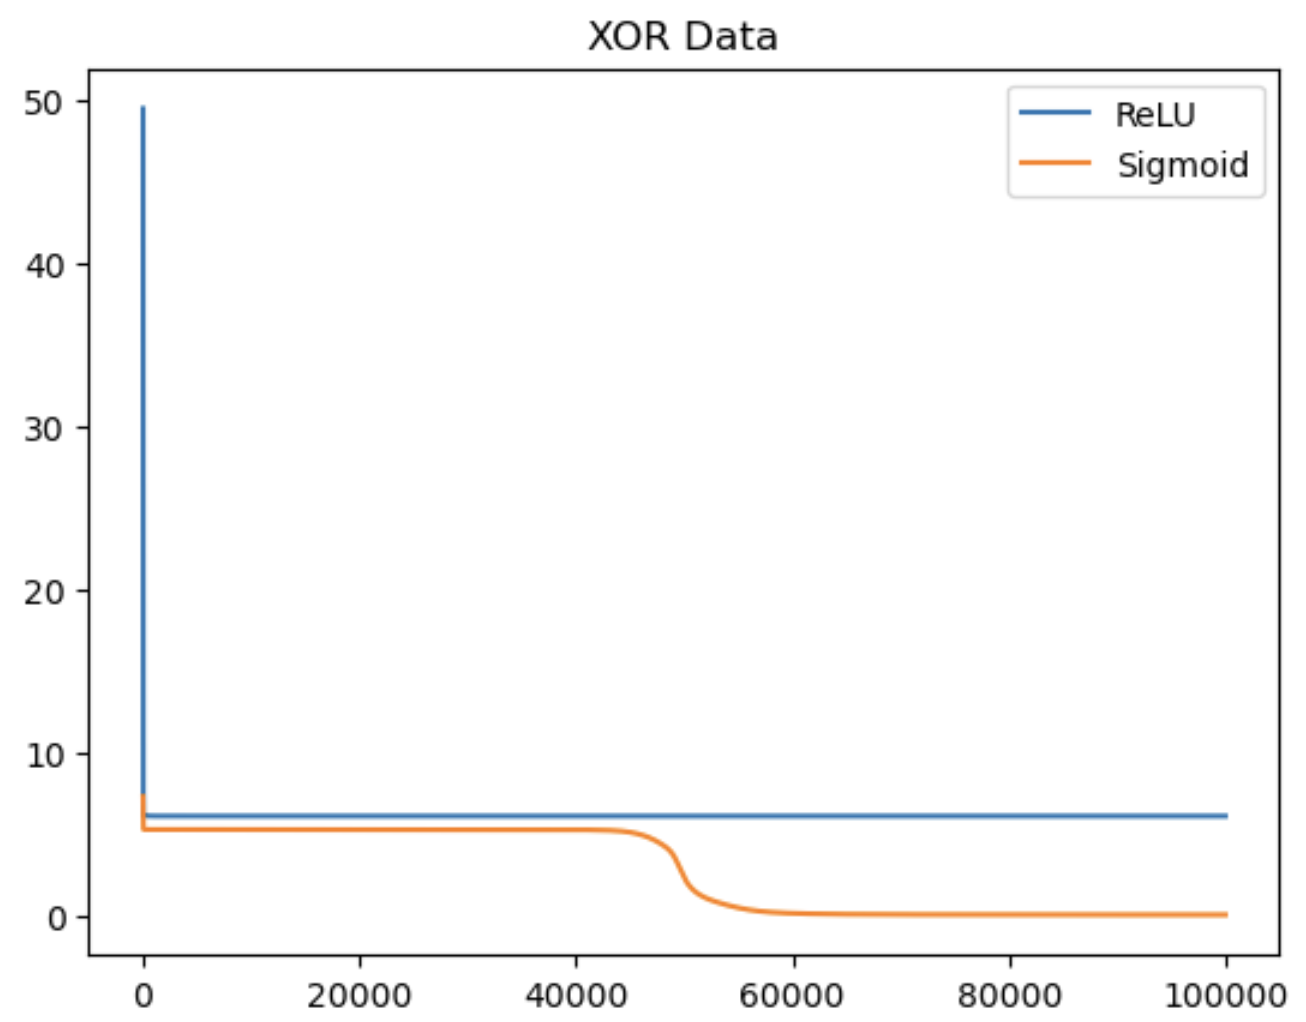
\includegraphics[width=7.5cm]{./imgs/xor_relu_loss.png}
    The loss of ReLU activation function is higher than Sigmoid activation function. 
    The accuracy of ReLU activation function is 86\% under linear data and 33\% under XOR data. 
    I suggest that ReLU can not bound the output to [0,1], so the model is harder to learn. \\
    
    \subsection{Different optimizers}
    Implement Adagrad and Momentum optimizers. \\
    Momentum optimizer: \\
    \[
    v_{t+1} = \beta v_t + \nabla L \quad
    W_{t+1} = W_t - \alpha v_{t+1}
    \]Adagrad optimizer: \\
    \[
    G_{t+1} = G_t + (\nabla L)^2 \quad
    W_{t+1} = W_t - \frac{\alpha}{\sqrt{G_{t+1}+\epsilon}} \nabla L
    \]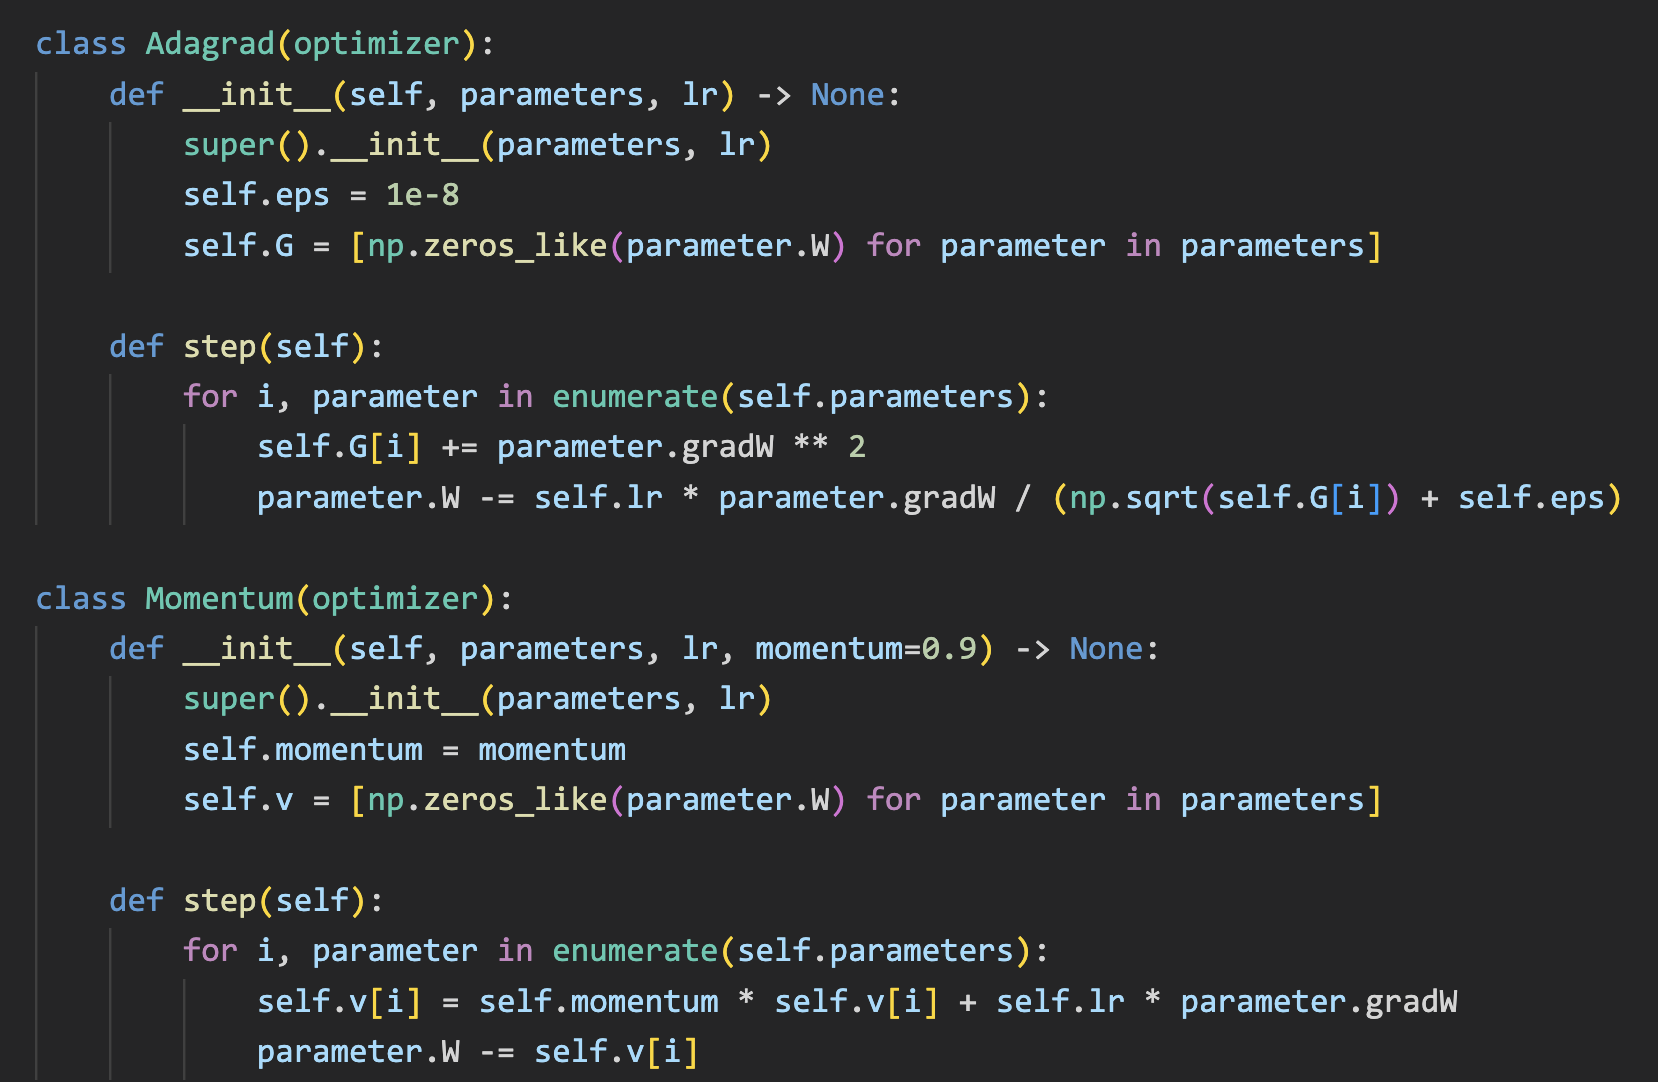
\includegraphics[width=10cm]{./imgs/opts.png} \\
    When the learning rate is 0.1, SGD and Adagrad can converge quikly and the accuracy is 100\% or near 100\%.
    But Momentum optimizer can not converge well and the accuracies are only 55\% and 52\%. \\
    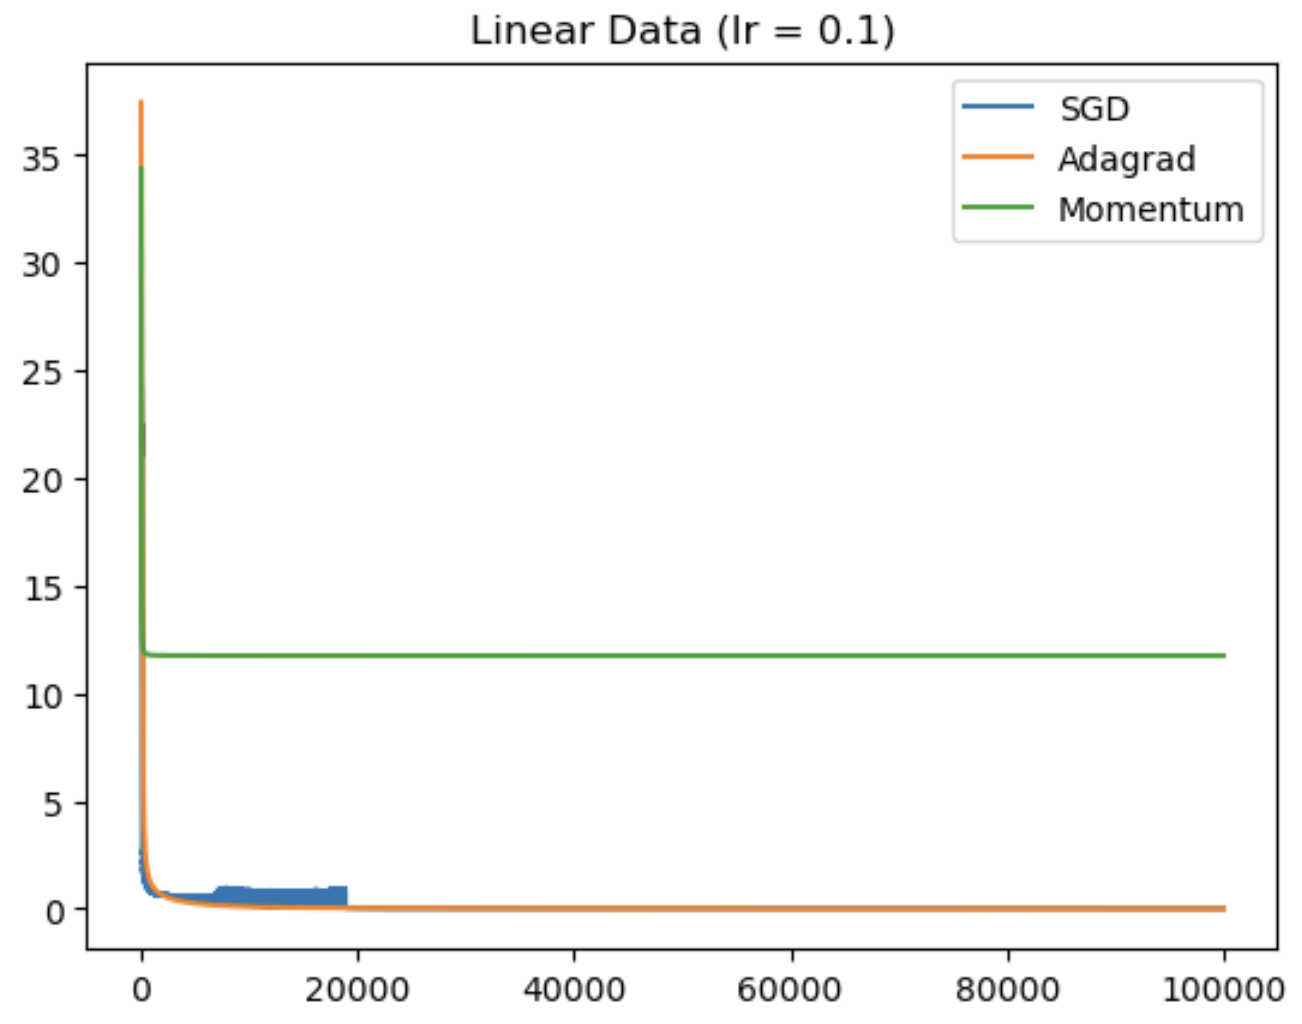
\includegraphics[width=7.5cm]{./imgs/linear_opt_0.1.png}
    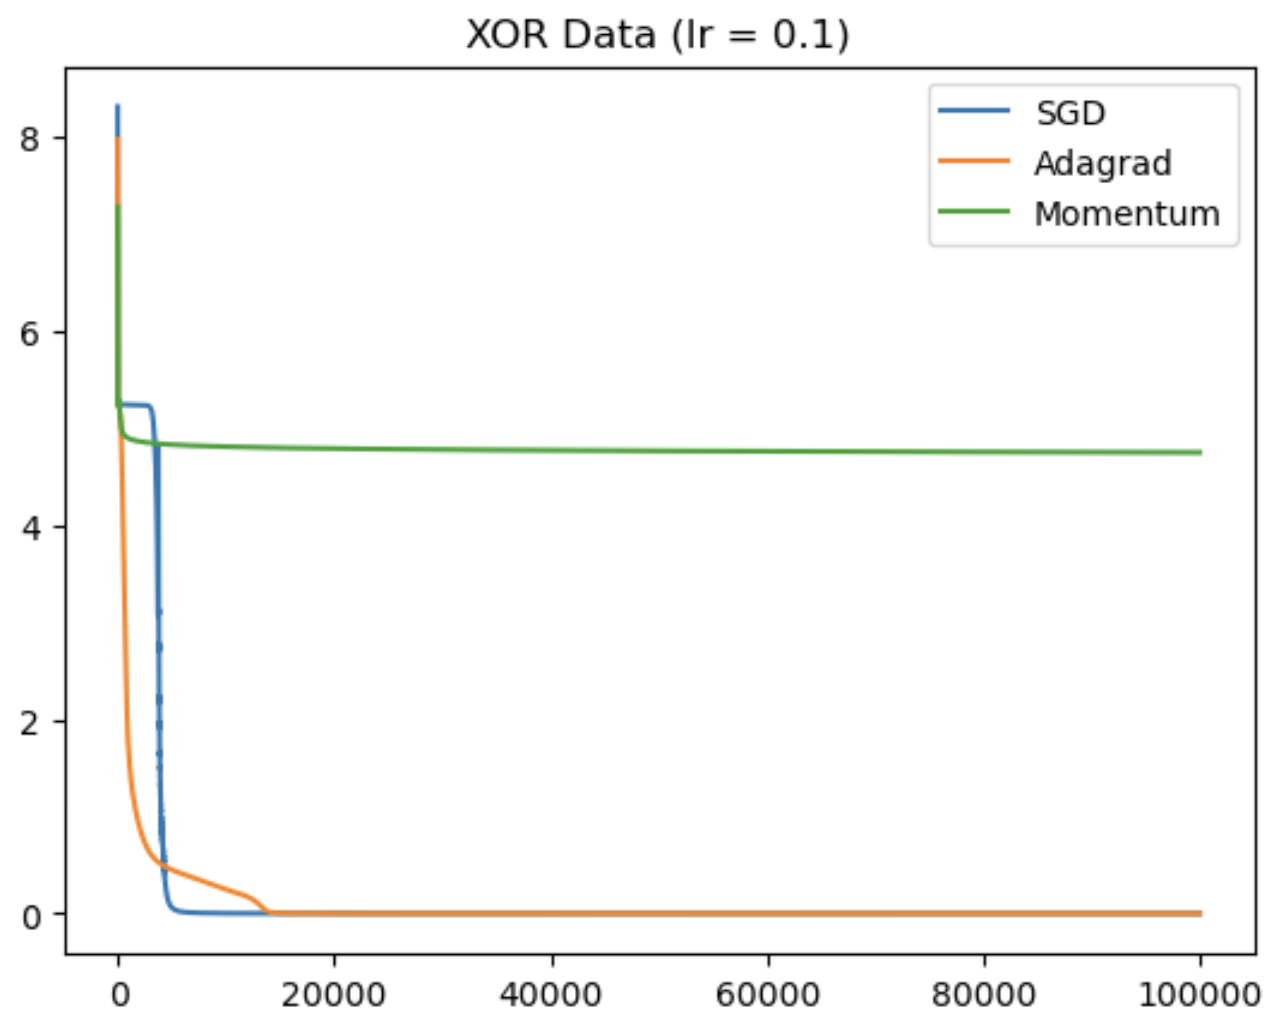
\includegraphics[width=7.5cm]{./imgs/xor_opt_0.1.png} \\
    When the learning rate is 0.001, Momentum can converge well under two datasets and the accuracy is 100\% or near 100\%.
    While SGD can perform well under linear data but not well under XOR data. Adagrad can not converge well under two datasets. 
    The accuracy of SGD is 100\% under linear data and 52\% under xor data. 
    The accuracy of Adagrad is 50\% and 52\%. \\
    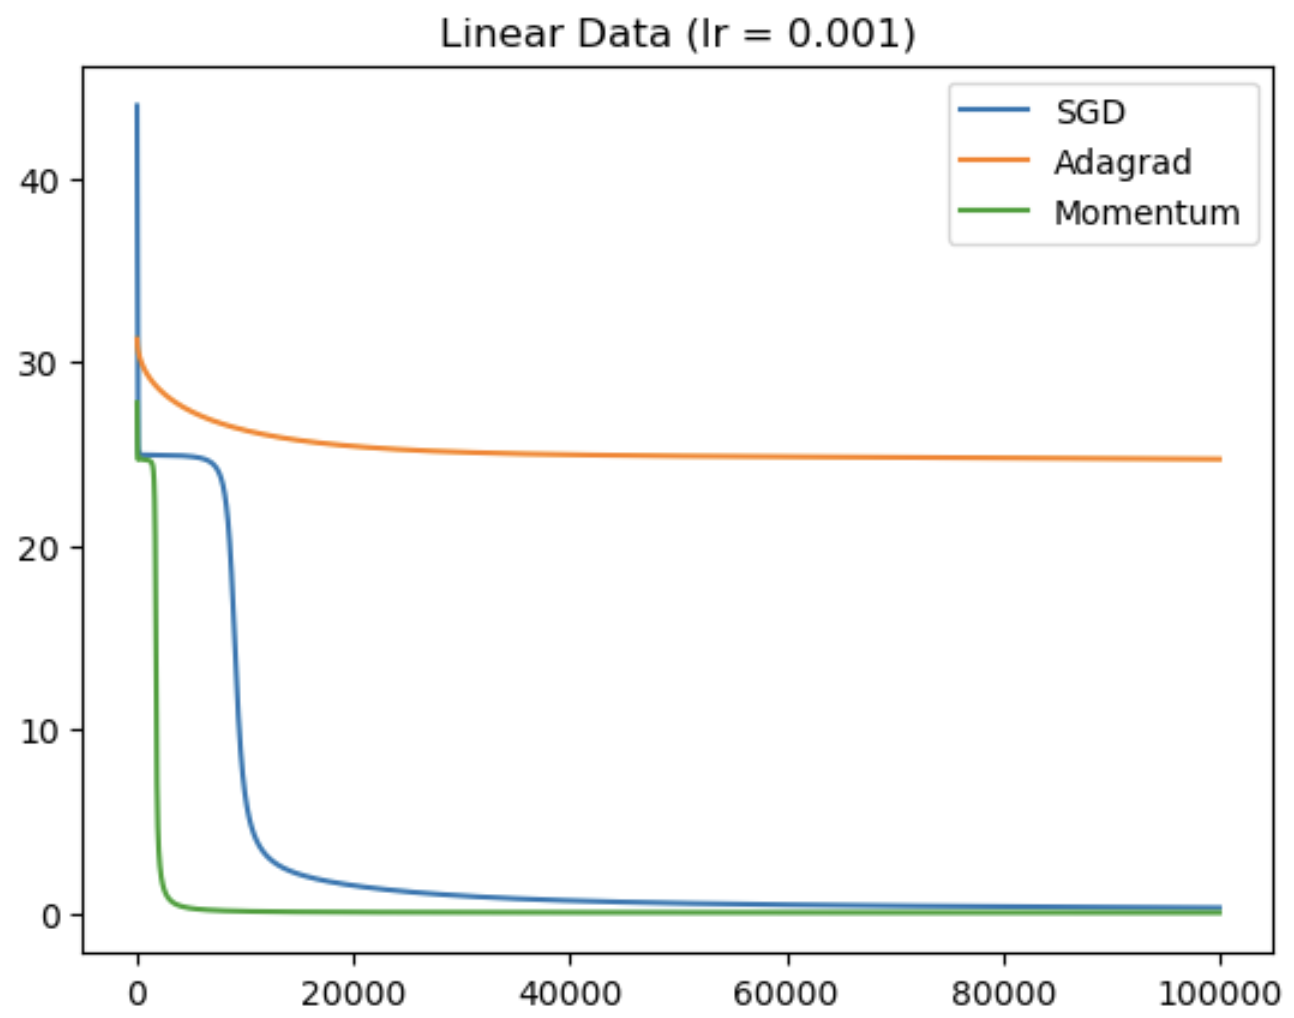
\includegraphics[width=7.5cm]{./imgs/linear_opt_0001.png}
    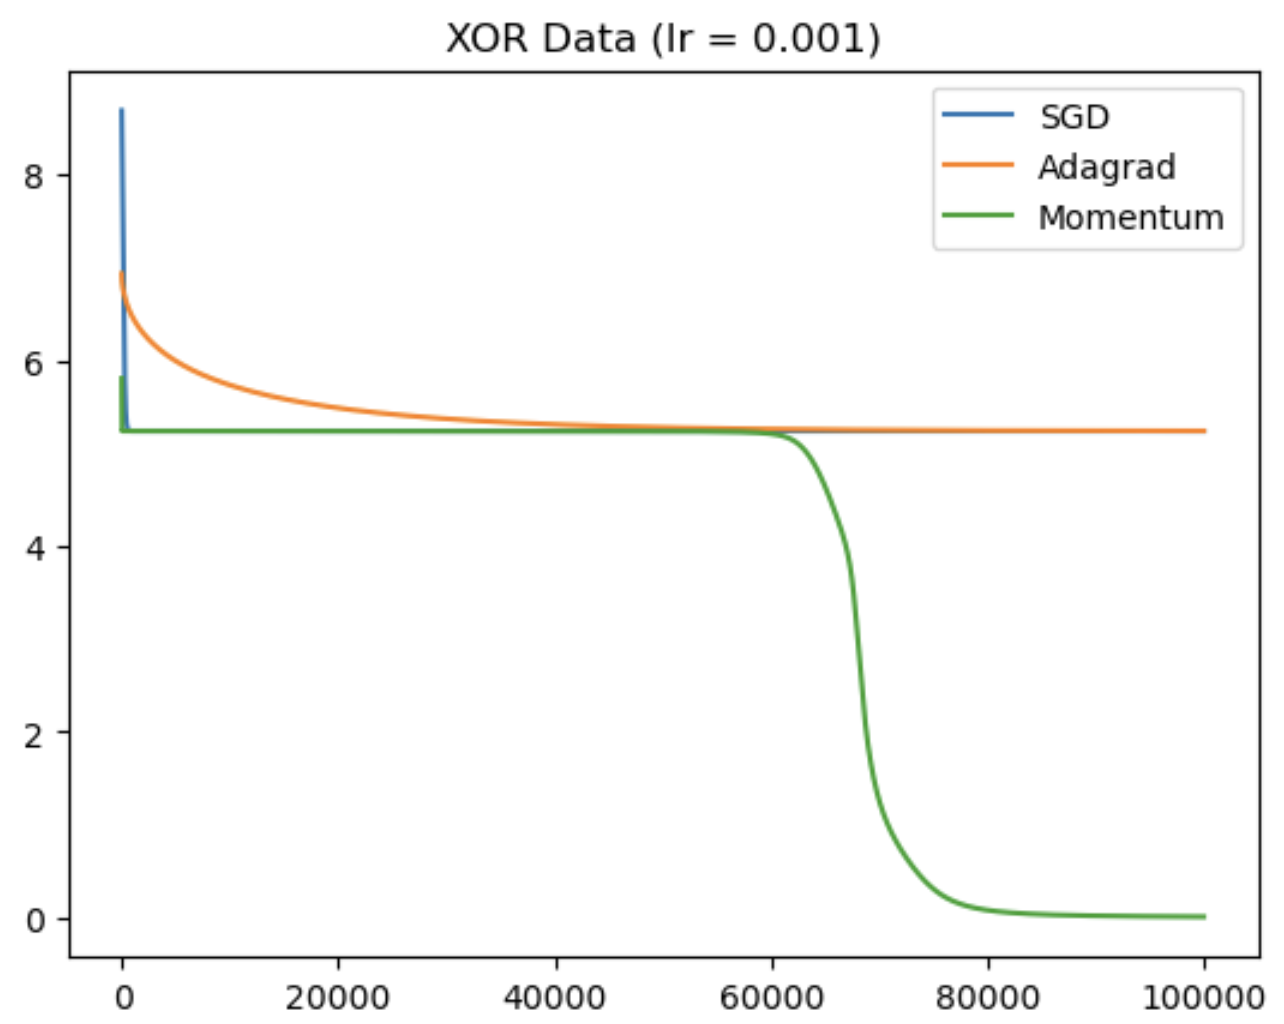
\includegraphics[width=7.5cm]{./imgs/xor_opt_0001.png}

\end{document}